\documentclass[11pt]{article}
\usepackage{amsmath,amssymb,amsmath,amsthm,amsfonts}
\usepackage{latexsym,graphicx}
\usepackage{fullpage,color}
\usepackage{url}
\usepackage[pdftex,bookmarks,colorlinks=true,citecolor=blue]{hyperref}
\usepackage{natbib}
\usepackage{graphicx,subfigure}
\usepackage{algorithm}
\usepackage{algorithmic}
\usepackage{listings}
\usepackage{xcolor}
\usepackage{framed}
\usepackage{color}

% \colorlet{shadecolor}{orange!15}
\colorlet{NextBlue}{orange!15!green!50!blue!75}

\numberwithin{equation}{section}

\pagestyle{plain}

\setlength{\oddsidemargin}{0in}
\setlength{\topmargin}{0in}
\setlength{\textwidth}{6.5in}
\setlength{\textheight}{8.5in}

\newtheorem{fact}{Fact}[section]
\newtheorem{question}{Question}[section]
\newtheorem{lemma}{Lemma}[section]
\newtheorem{theorem}[lemma]{Theorem}
\newtheorem{assumption}[lemma]{Assumption}
\newtheorem{corollary}[lemma]{Corollary}
\newtheorem{prop}[lemma]{Proposition}
\newtheorem{claim}{Claim}[section]
\newtheorem{remark}{Remark}[section]
\newtheorem{definition}{Definition}[section]
\newtheorem{prob}{Problem}[section]
\newtheorem{conjecture}{Conjecture}[section]
\newtheorem{property}{Property}[section]

\def\A{{\bf A}}
\def\a{{\bf a}}
\def\B{{\bf B}}
\def\bb{{\bf b}}
\def\C{{\bf C}}
\def\c{{\bf c}}
\def\D{{\bf D}}
\def\d{{\bf d}}
\def\E{{\bf E}}
\def\e{{\bf e}}
\def\F{{\bf F}}
\def\f{{\bf f}}
\def\g{{\bf g}}
\def\h{{\bf h}}
\def\G{{\bf G}}
\def\H{{\bf H}}
\def\I{{\bf I}}
\def\K{{\bf K}}
\def\k{{\bf k}}
\def\LL{{\bf L}}
\def\M{{\bf M}}
\def\m{{\bf m}}
\def\N{{\bf N}}
\def\n{{\bf n}}
\def\PP{{\bf P}}
\def\pp{{\bf p}}
\def\Q{{\bf Q}}
\def\q{{\bf q}}
\def\R{{\bf R}}
\def\rr{{\bf r}}
\def\S{{\bf S}}
\def\s{{\bf s}}
\def\T{{\bf T}}
\def\tt{{\bf t}}
\def\U{{\bf U}}
\def\u{{\bf u}}
\def\V{{\bf V}}
\def\v{{\bf v}}
\def\W{{\bf W}}
\def\w{{\bf w}}
\def\X{{\bf X}}
\def\x{{\bf x}}
\def\Y{{\bf Y}}
\def\y{{\bf y}}
\def\Z{{\bf Z}}
\def\z{{\bf z}}
\def\0{{\bf 0}}
\def\1{{\bf 1}}



\def\AM{{\mathcal A}}
\def\CM{{\mathcal C}}
\def\DM{{\mathcal D}}
\def\EM{{\mathcal E}}
\def\GM{{\mathcal G}}
\def\FM{{\mathcal F}}
\def\IM{{\mathcal I}}
\def\JM{{\mathcal J}}
\def\KM{{\mathcal K}}
\def\LM{{\mathcal L}}
\def\NM{{\mathcal N}}
\def\OM{{\mathcal O}}
\def\PM{{\mathcal P}}
\def\SM{{\mathcal S}}
\def\TM{{\mathcal T}}
\def\UM{{\mathcal U}}
\def\VM{{\mathcal V}}
\def\WM{{\mathcal W}}
\def\XM{{\mathcal X}}
\def\YM{{\mathcal Y}}
\def\RB{{\mathbb R}}
\def\RBmn{{\RB^{m\times n}}}
\def\EB{{\mathbb E}}
\def\PB{{\mathbb P}}

\def\TX{\tilde{\bf X}}
\def\TA{\tilde{\bf A}}
\def\tx{\tilde{\bf x}}
\def\ty{\tilde{\bf y}}
\def\TZ{\tilde{\bf Z}}
\def\tz{\tilde{\bf z}}
\def\hd{\hat{d}}
\def\HD{\hat{\bf D}}
\def\hx{\hat{\bf x}}
\def\nysA{{\tilde{\A}_c^{\textrm{nys}}}}

\def\alp{\mbox{\boldmath$\alpha$\unboldmath}}
\def\bet{\mbox{\boldmath$\beta$\unboldmath}}
\def\epsi{\mbox{\boldmath$\epsilon$\unboldmath}}
\def\etab{\mbox{\boldmath$\eta$\unboldmath}}
\def\ph{\mbox{\boldmath$\phi$\unboldmath}}
\def\pii{\mbox{\boldmath$\pi$\unboldmath}}
\def\Ph{\mbox{\boldmath$\Phi$\unboldmath}}
\def\Ps{\mbox{\boldmath$\Psi$\unboldmath}}
\def\ps{\mbox{\boldmath$\psi$\unboldmath}}
\def\tha{\mbox{\boldmath$\theta$\unboldmath}}
\def\Tha{\mbox{\boldmath$\Theta$\unboldmath}}
\def\muu{\mbox{\boldmath$\mu$\unboldmath}}
\def\Si{\mbox{\boldmath$\Sigma$\unboldmath}}
\def\si{\mbox{\boldmath$\sigma$\unboldmath}}
\def\Gam{\mbox{\boldmath$\Gamma$\unboldmath}}
\def\Lam{\mbox{\boldmath$\Lambda$\unboldmath}}
\def\De{\mbox{\boldmath$\Delta$\unboldmath}}
\def\Ome{\mbox{\boldmath$\Omega$\unboldmath}}
\def\Pii{\mbox{\boldmath$\Pi$\unboldmath}}
\def\varepsi{\mbox{\boldmath$\varepsilon$\unboldmath}}
\newcommand{\ti}[1]{\tilde{#1}}
\def\Ncal{\mathcal{N}}
\def\argmax{\mathop{\rm argmax}}
\def\argmin{\mathop{\rm argmin}}

\def\ALG{{\AM_{\textrm{col}}}}

\def\mean{\mathsf{mean}}
\def\std{\mathsf{std}}
\def\bias{\mathsf{bias}}
\def\var{\mathsf{var}}
\def\sgn{\mathsf{sgn}}
\def\tr{\mathsf{tr}}
\def\rk{\mathrm{rank}}
\def\nnz{\mathsf{nnz}}
\def\poly{\mathrm{poly}}
\def\diag{\mathsf{diag}}
\def\Diag{\mathsf{Diag}}
\def\const{\mathrm{Const}}
\def\st{\mathsf{s.t.}}
\def\vect{\mathsf{vec}}
\def\sech{\mathrm{sech}}
\def\sigmoid{\mathsf{sigmoid}}

\newcommand{\red}[1]{{\color{red}#1}}



\def\argmax{\mathop{\rm argmax}}
\def\argmin{\mathop{\rm argmin}}

\newenvironment{note}[1]{\medskip\noindent \textbf{#1:}}%
        {\medskip}


\newcommand{\etal}{{\em et al.}\ }
\newcommand{\assign}{\leftarrow}
\newcommand{\eps}{\epsilon}

\newcommand{\opt}{\textrm{\sc OPT}}
\newcommand{\script}[1]{\mathcal{#1}}
\newcommand{\ceil}[1]{\lceil #1 \rceil}
\newcommand{\floor}[1]{\lfloor #1 \rfloor}



\lstset{ %
extendedchars=false,            % Shutdown no-ASCII compatible
language=Python,                % choose the language of the code
xleftmargin=1em,
xrightmargin=1em,
basicstyle=\footnotesize,    % the size of the fonts that are used for the code
tabsize=3,                            % sets default tabsize to 3 spaces
numbers=left,                   % where to put the line-numbers
numberstyle=\tiny,              % the size of the fonts that are used for the line-numbers
stepnumber=1,                   % the step between two line-numbers. If it's 1 each line
                                % will be numbered
numbersep=5pt,                  % how far the line-numbers are from the code   %
keywordstyle=\color[rgb]{0,0,1},                % keywords
commentstyle=\color[rgb]{0.133,0.545,0.133},    % comments
stringstyle=\color[rgb]{0.627,0.126,0.941},      % strings
backgroundcolor=\color{white}, % choose the background color. You must add \usepackage{color}
showspaces=false,               % show spaces adding particular underscores
showstringspaces=false,         % underline spaces within strings
showtabs=false,                 % show tabs within strings adding particular underscores
frame=single,                 % adds a frame around the code
%captionpos=b,                   % sets the caption-position to bottom
breaklines=true,                % sets automatic line breaking
breakatwhitespace=false,        % sets if automatic breaks should only happen at whitespace
%title=\lstname,                 % show the filename of files included with \lstinputlisting;
%                                % also try caption instead of title
mathescape=true,escapechar=?    % escape to latex with ?..?
escapeinside={\%*}{*)},         % if you want to add a comment within your code
%columns=fixed,                  % nice spacing
%morestring=[m]',                % strings
%morekeywords={%,...},%          % if you want to add more keywords to the set
%    break,case,catch,continue,elseif,else,end,for,function,global,%
%    if,otherwise,persistent,return,switch,try,while,...},%
}


\begin{document}

%\setlength{\fboxrule}{.5mm}\setlength{\fboxsep}{1.2mm}
%\newlength{\boxlength}\setlength{\boxlength}{\textwidth}
%\addtolength{\boxlength}{-4mm}


\title{Poison Frogs! Targeted Clean-Label Poisoning
Attacks on Neural Networks}

\author{\textbf{W. Ronny Huang \etal} \\ University of Maryland\\homepage: \url{https://wrhuang.com/}}

%\date{ }

\maketitle

\begin{abstract}
% This lecture note describes synchronous parallel accelerated gradient descent (AGD) for empirical risk minimization ERM.
% We first describe AGD for solving ERM.
% We then show how to parallelize AGD; in particular, we assume there is a central parameter server and the data are partitioned among the worker nodes.
% We finally use Python to write a simulator that mimics synchronous parallel AGD.

This paper is about poisoning attack, wherein the attacker adds examples to the training set to manipulate the behavior of the model at the test time.

An attacker add a seemingly innocuous image, which is properly labeled to a training set and control the identity of a chosen sample at test time. The attacker dose not need to control the labelling function.

Method for crafting poisons: Optimization-based method.

For transfer learning: One single poison image can control classifier behavior
For full end-to-end training: (1) Optimization,(2) diversity of poison instances, and (3) watermarking.
\end{abstract}




\section{Brief introduction of the proposed \textit{clean-label} attacks} \label{sec:optimization}

\begin{itemize}
    \item clean-label attacks: the attacker’s injected training examples are cleanly labeled by a certified authority. {\color{blue} The poisoning sample is labelled as it looks like (similar to base sample ) and its features are similar to another sample from another class (target sample).}
    \item Assumption: The attacker has no knowledge of the training data but has knowledge of the model and its parameters.{\color{blue}{ (Many classic networks pretrained on standard datasets, such as ResNet or Inception trained on ImageNet.)}}
    \item The attacker's goal: Cause the retained network to misclassify a specical test instance from one class as another class of her choice.{\color{blue}{ Retrain the network on the augmented data set that includes poison instances.}}
    \item State-of-art poisoning defenses that measure the performance impact of training instances ineffective.{\color{blue}{ Besides the intended misprediction on the target, the performance degradation on the victim classifier is not noticeable.}}
\end{itemize}


\section{A simple clean-label attack}

\begin{enumerate}
    \item {\color{red}{(Attacker)}} Choose a \textit{target instance} from the test set. If the poisoning attack is successful, this example will be misclassified during test time.
    \item {\color{red}{(Attacker)}} Sample a \textit{base instance} from the base class and make imperceptible changes to it to craft \textit{a poison instance}. 
    \item Inject the poisoning example into the training data.
    \item Train the model on the poisoned dataset (clean dataset + poison instances).
\end{enumerate}

\subsection{Crafting poison data via feature collisions}

Find an example $\x$: 

\begin{enumerate}
    \item "collides" with the {\color{red}target} in {\color{red}{feature space}}.
    \item close to the {\color{blue}base instance} $\bb$ in {\color{blue}input space}.
\end{enumerate}

The objective function:

\begin{equation}
    \mathbf{p}= \underset{\mathbf{x}}{\operatorname{argmin}}\underbrace{\|f(\mathbf{x})-f(\mathbf{t})\|_{2}^{2}}_{\text{Close to target in feature Space}} +\beta \underbrace{\|\mathbf{x}-\mathbf{b}\|_{2}^{2}}_{\text{Close to base in pixel Space}}
    \label{eq:poison data}
\end{equation}

$f(x)$: \text{feature space representation of the input } $\x$. The activation of the penultimate layer(before the softmax layer).

% The right-most term of \equationautorefname{\ref{eq:poison data}} cause $\pp$ to appear like a base class instance to a human labeler($\beta$ controls the degree) and be labelled as such.

% The first term cause the poison instance to move toward the target instance in feature space and get embedded in the target class distribution.

\colorbox{NextBlue!20}{\textbf{Clean model:}}
misclassify the poison as a target;

\colorbox{orange!15}{\textbf{Retrain the model on the clean $+$ poison instance:}}
misclassify the target into the base class during test time.

\subsection{Optimization procedure}

\textbf{Forward-backward-splitting iterative procedure:}

\begin{enumerate}
    \item (forward) gradient descent update to minimize the $L_2$ distance to the target instance in feature space.
    \item (backward) minimize the Frobenius distance from the base instance in input space.
\end{enumerate}

\begin{figure}[!h]
	\centering
	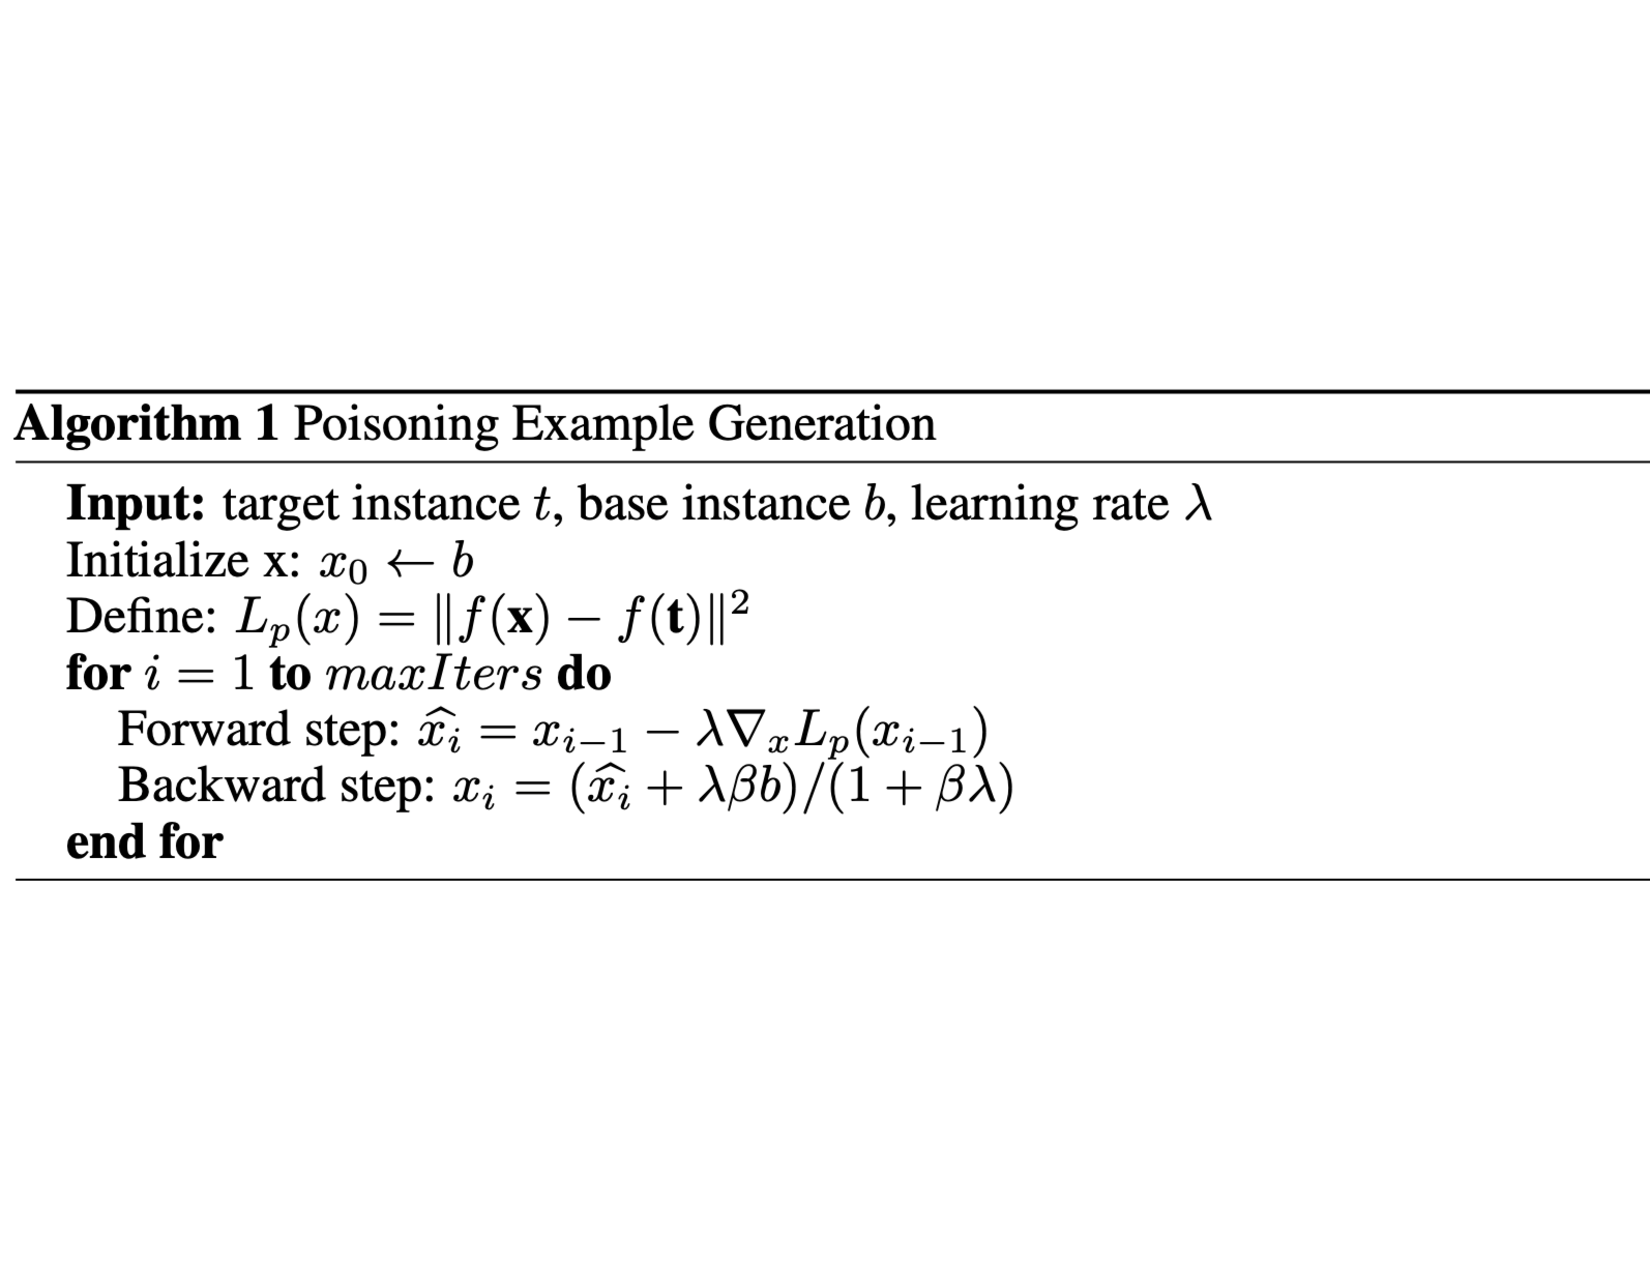
\includegraphics[width=17cm]{figures/alg1.pdf}
% 	\caption{Illustration of parallel AGD.}
	\label{fig:alg1}
\end{figure}

\colorbox{orange!15}{backward step:}

\begin{align*}
    x_i &= \hat{x_i} - \beta \lambda (x_i - b)\\
    x_i &= \hat{x_i} - \beta \lambda x_i - \beta \lambda b\\
    x_i + \beta \lambda x_i &= \hat{x_i} + \beta \lambda b\\
    x_i &= \frac{\hat{x_i} + \beta \lambda b}{1 + \beta \lambda x_i}
\end{align*}

\section{Experiment on different settings}

\subsection{Transfer learning}

\begin{itemize}
    \item Standard, pre-trained net is used
    \item “Feature extraction”layers frozen
    \item classification layers re-trained
    \item Common practice in industry
\end{itemize}

\colorbox{orange!15}{A one-shot kill attack}

\begin{itemize}
    \item select both target and base instance from the test set to craft a poison instance
    \item adding just one poison instance to the training set
\end{itemize}

\begin{figure}[!h]
	\centering
	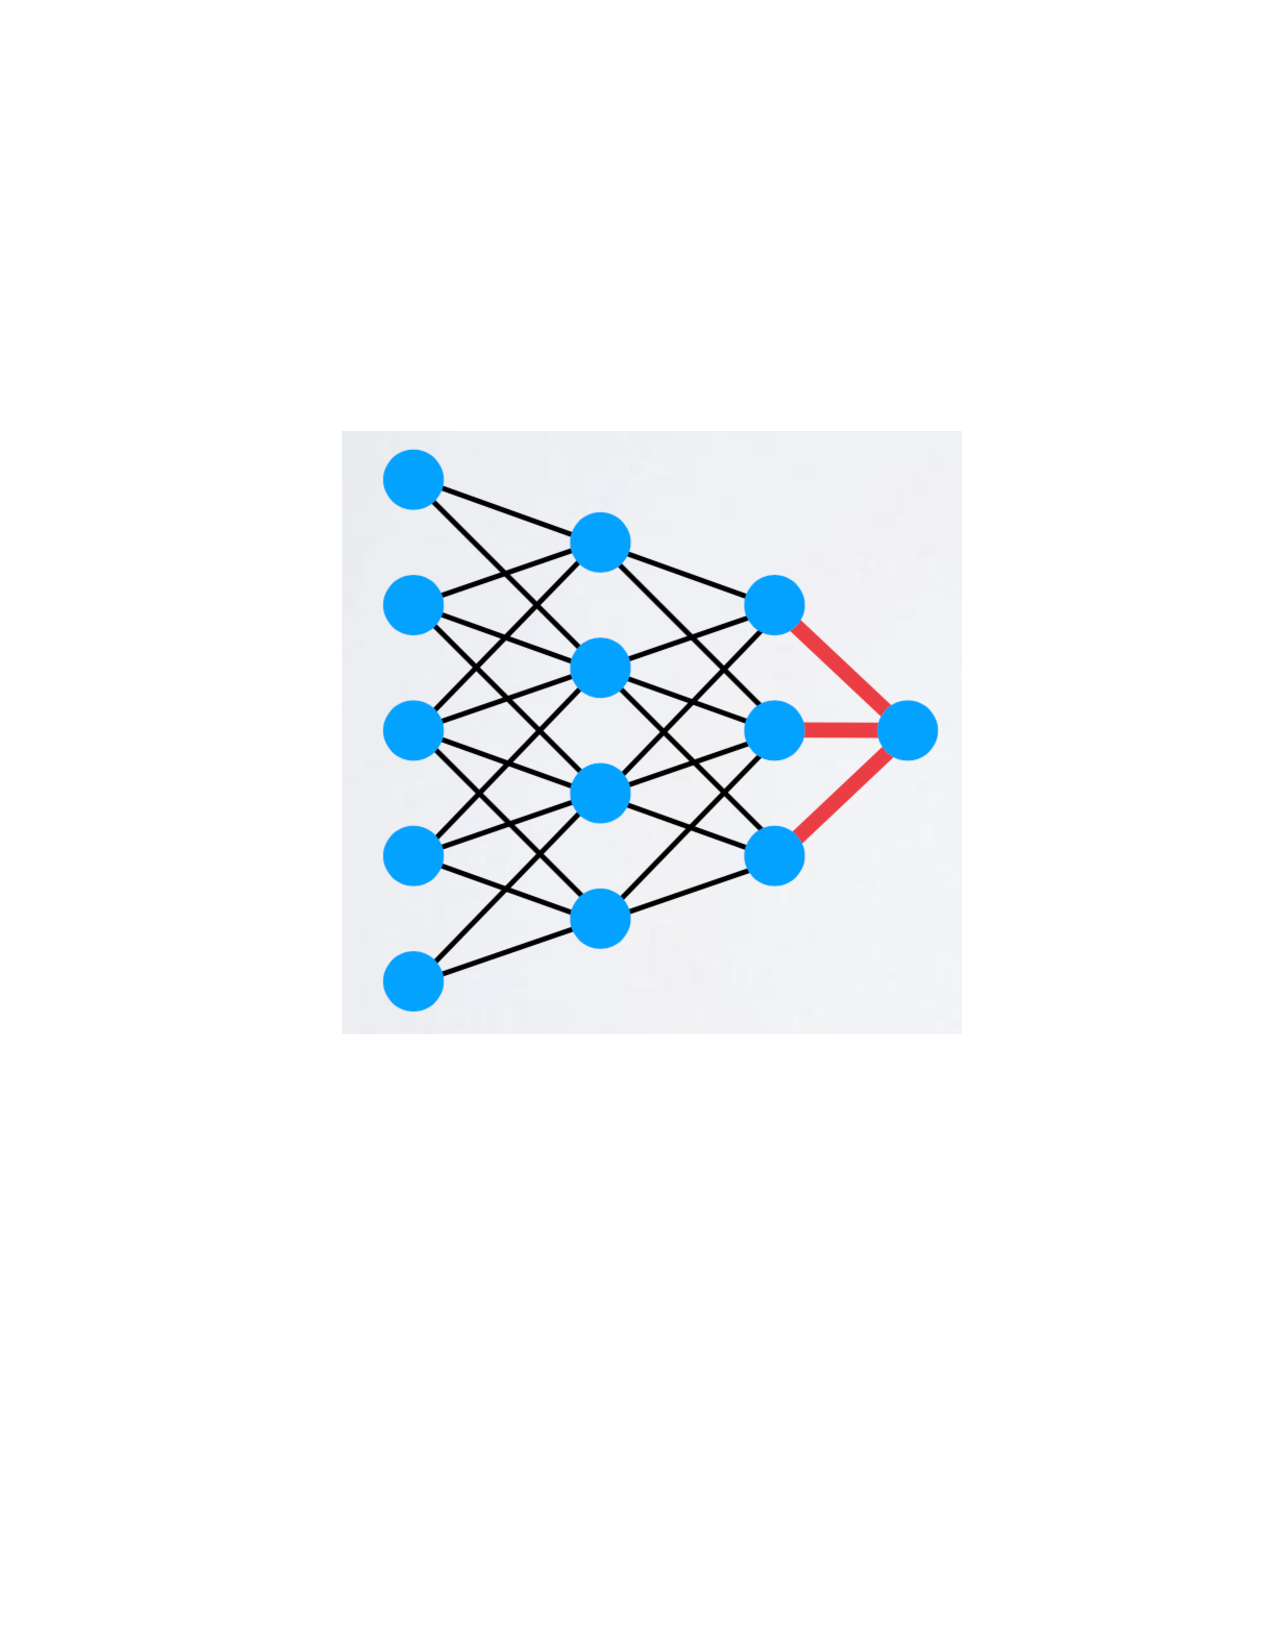
\includegraphics[width=6cm]{figures/transfer.pdf}
	\caption{Transfer learning}
	\label{fig:transfer}
\end{figure}


\begin{figure}[!h]
	\centering
	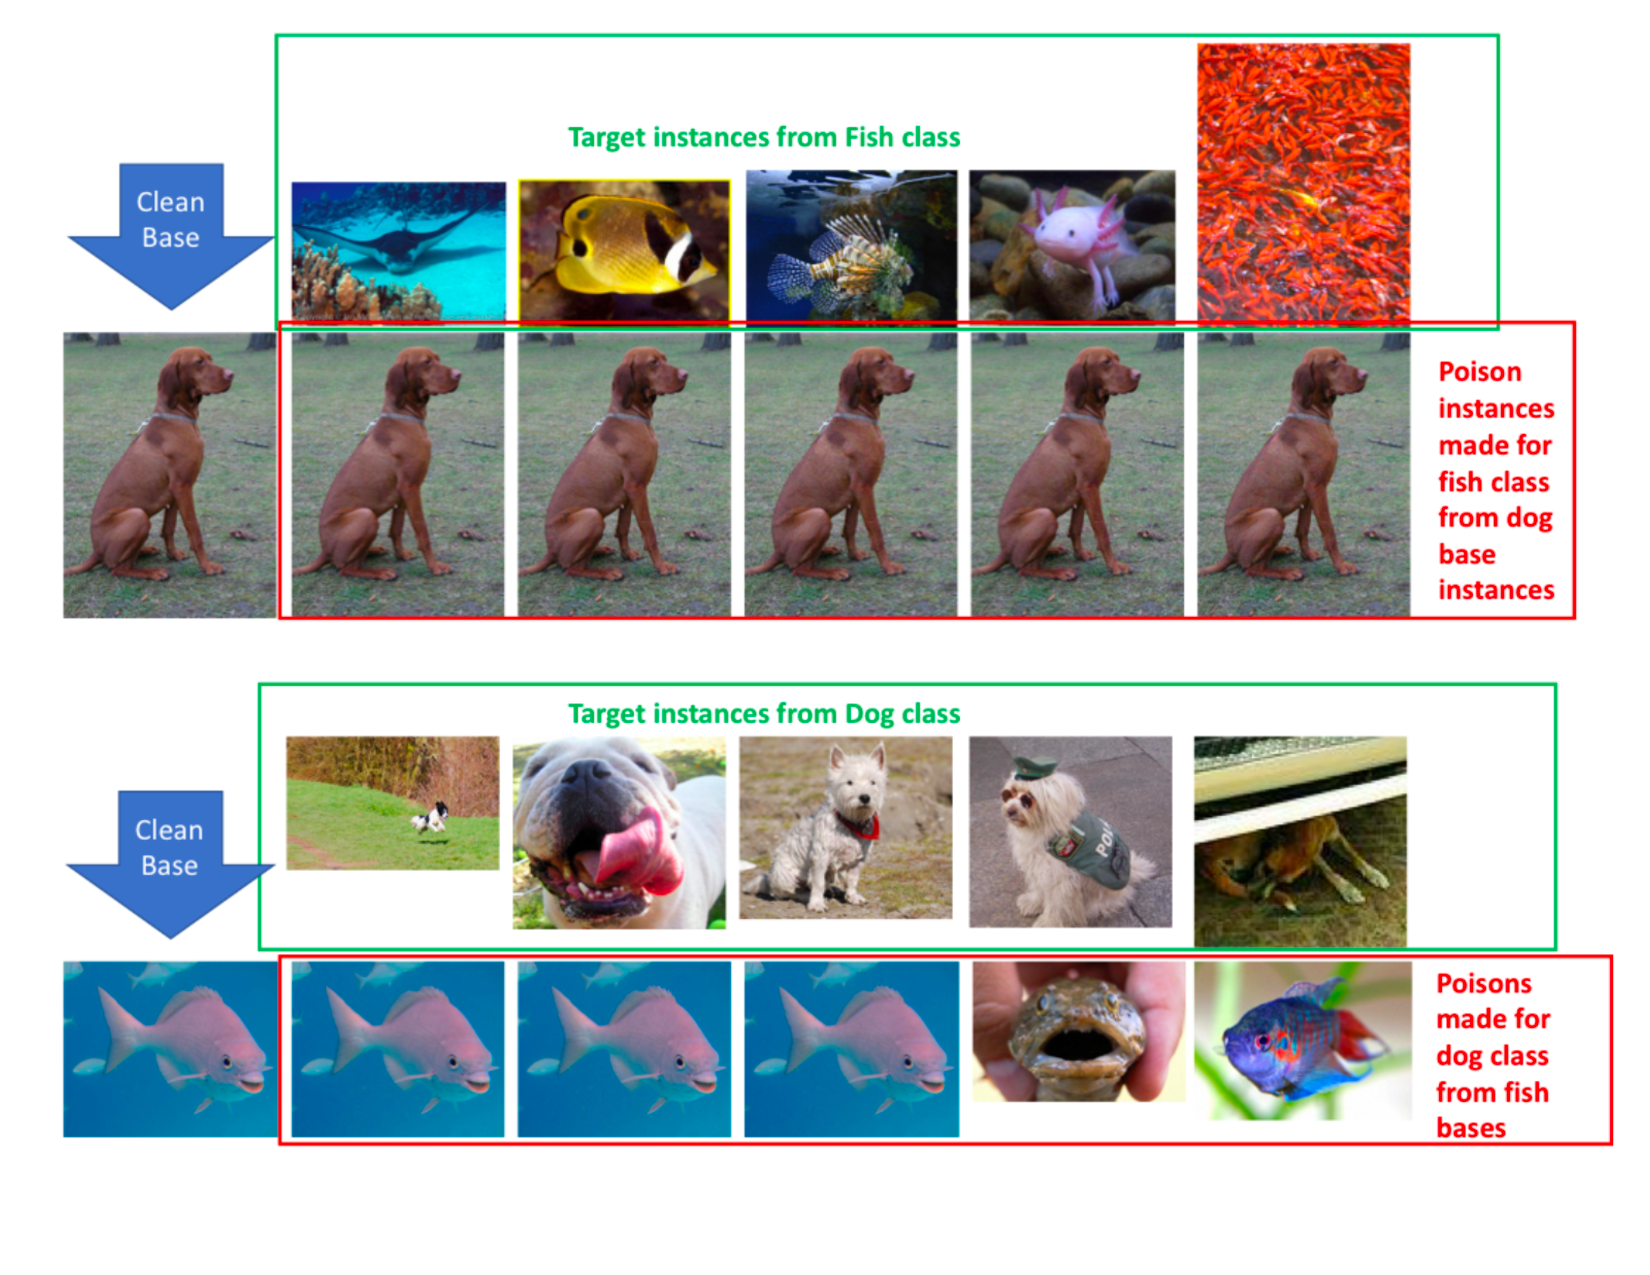
\includegraphics[width=15cm]{figures/P_instances.pdf}
	\caption{Sample target and poison instances}
	\label{fig:P_instances}
\end{figure}

\begin{figure}[!h]
	\centering
	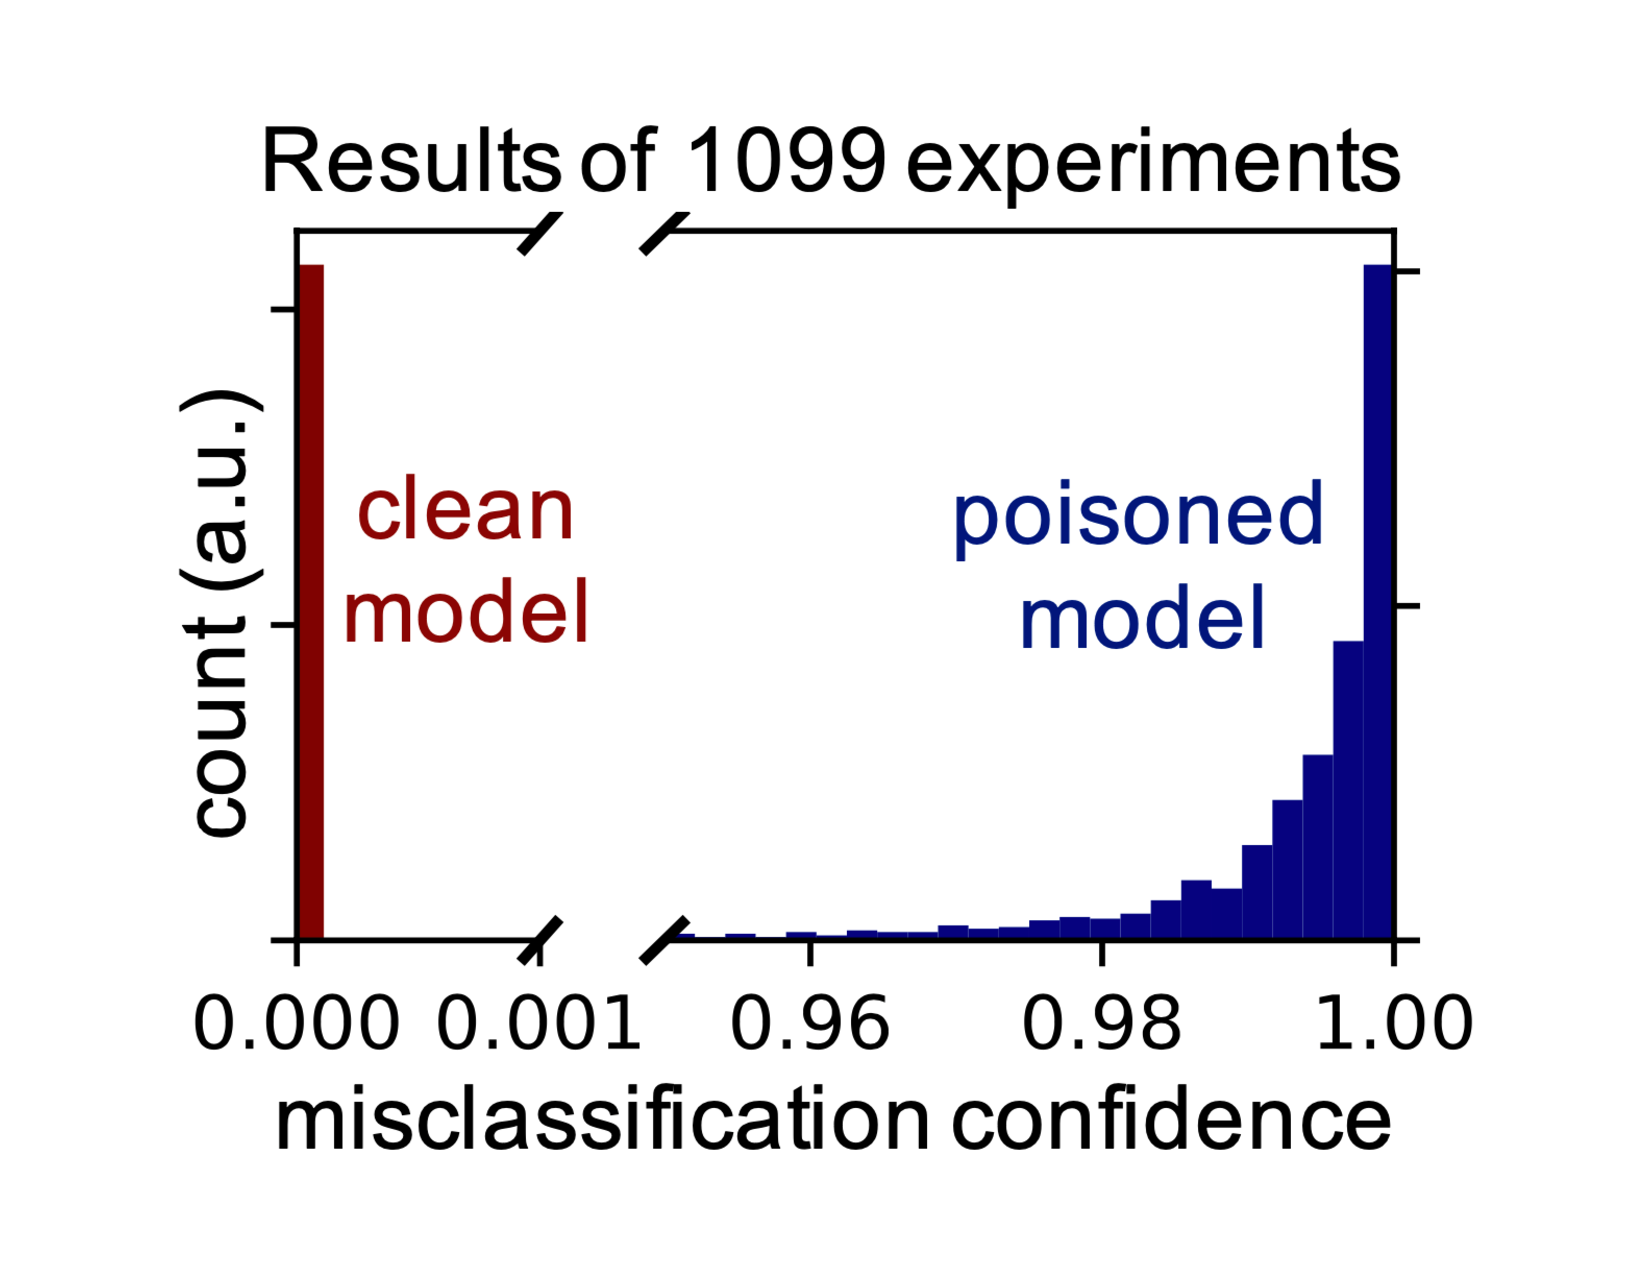
\includegraphics[width=8cm]{figures/P_misclassify.pdf}
	\caption{When trained on a poisoned dataset, the target instances get misclassified with high confidence.}
	\label{fig:P_misclassify}
\end{figure}

\begin{figure}[!h]
	\centering
	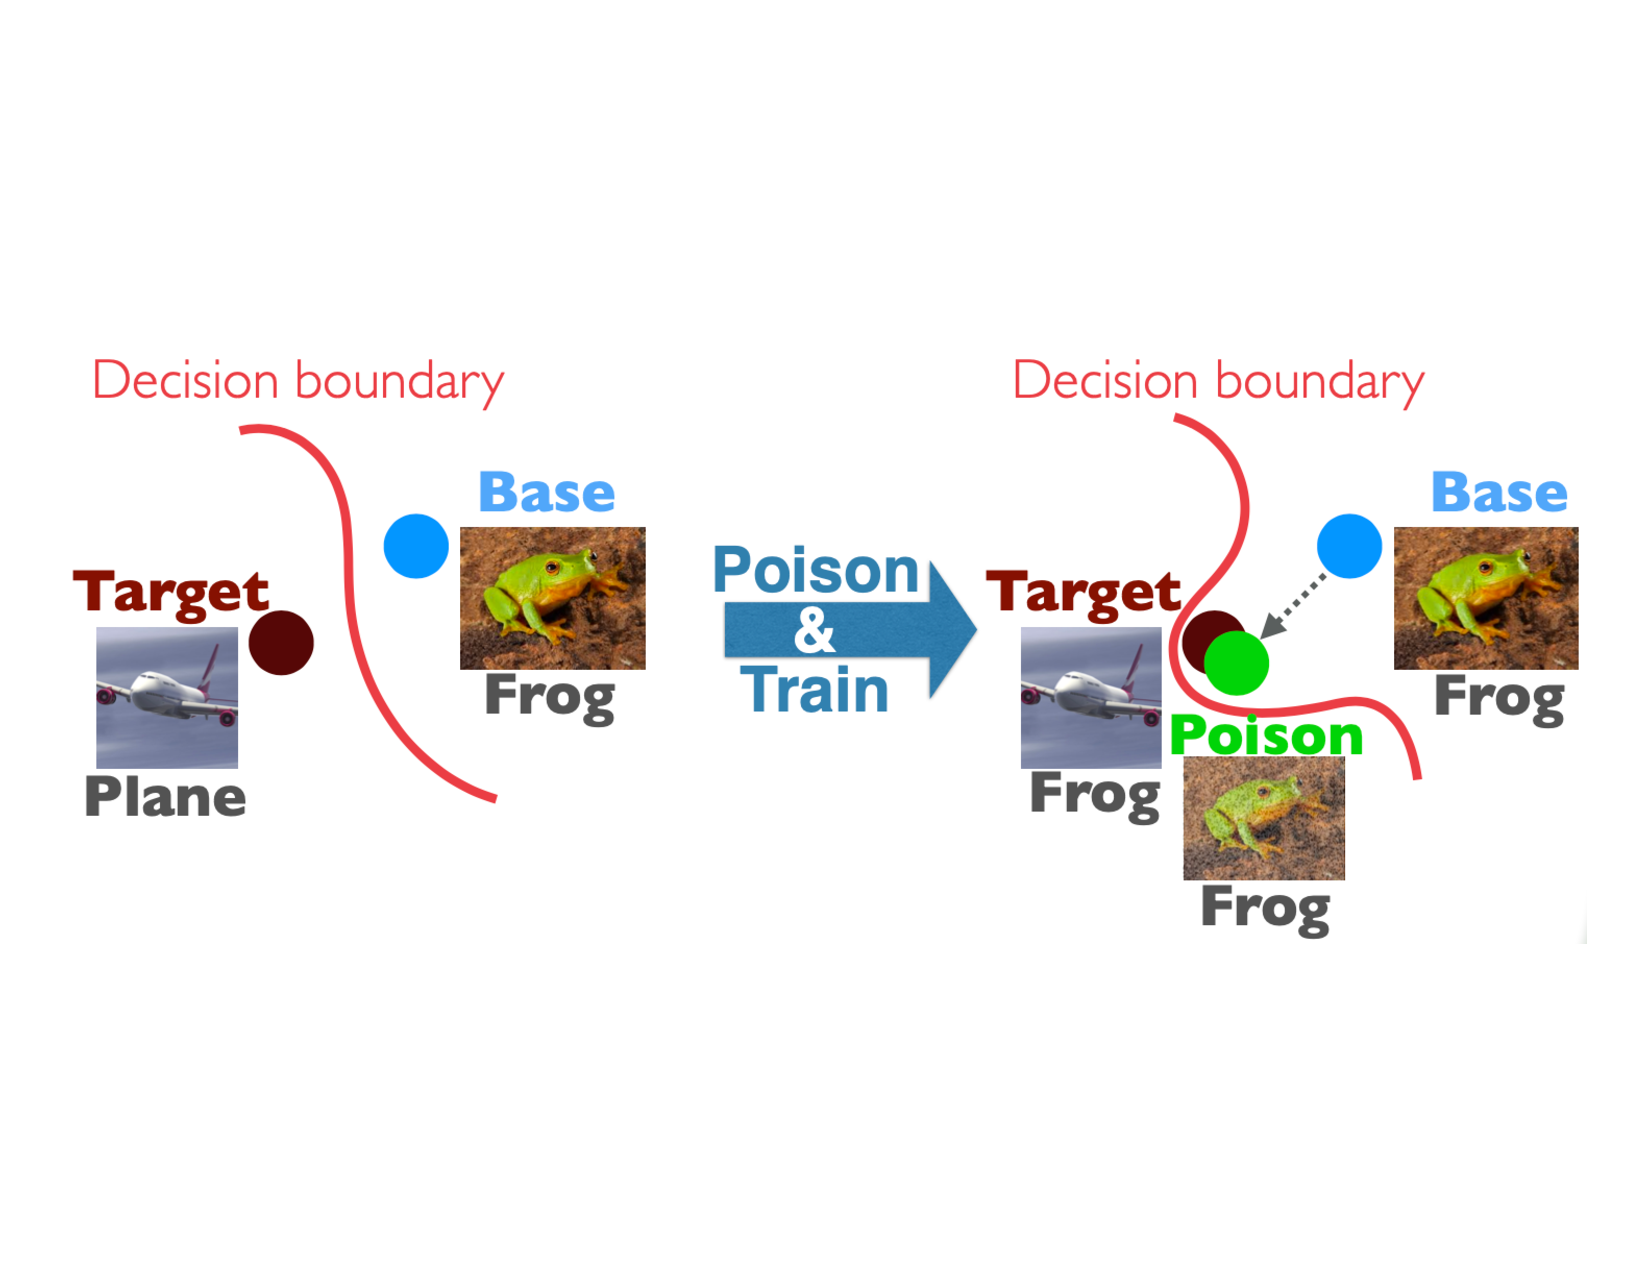
\includegraphics[width=14cm]{figures/One_boundary.pdf}
	\caption{When trained on a poisoned dataset, the decision boundary changes.}
	\label{fig:One_boundary}
\end{figure}

\subsection{End-to-end retraining}
\colorbox{orange!15}{Multiple poisons required}

\begin{itemize}
    \item Pre-trained net is used
    \item All-layers are re-trained
\end{itemize}

\begin{figure}[!h]
	\centering
	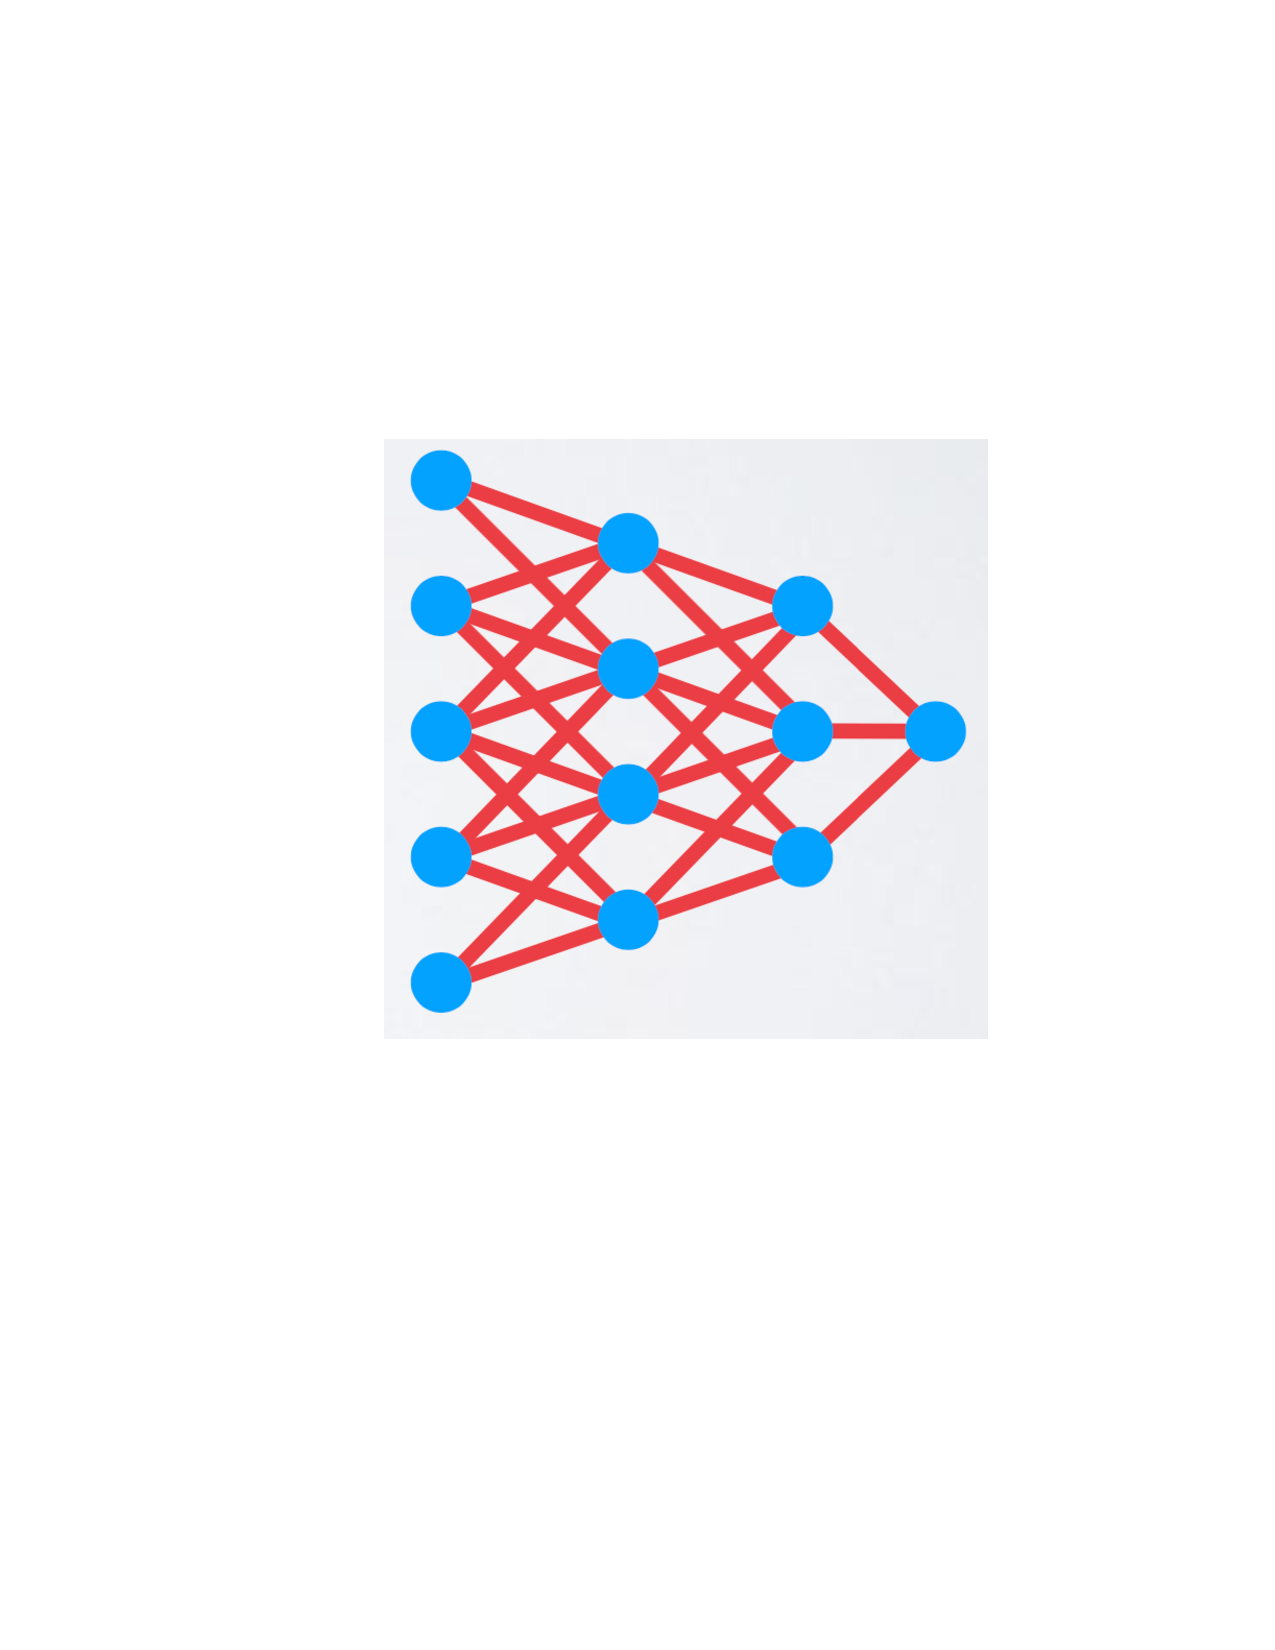
\includegraphics[width=6cm]{figures/end2end.pdf}
	\caption{End-to-end training.}
	\label{fig:P_misclassify}
\end{figure}

\begin{figure}[H]
	\centering
	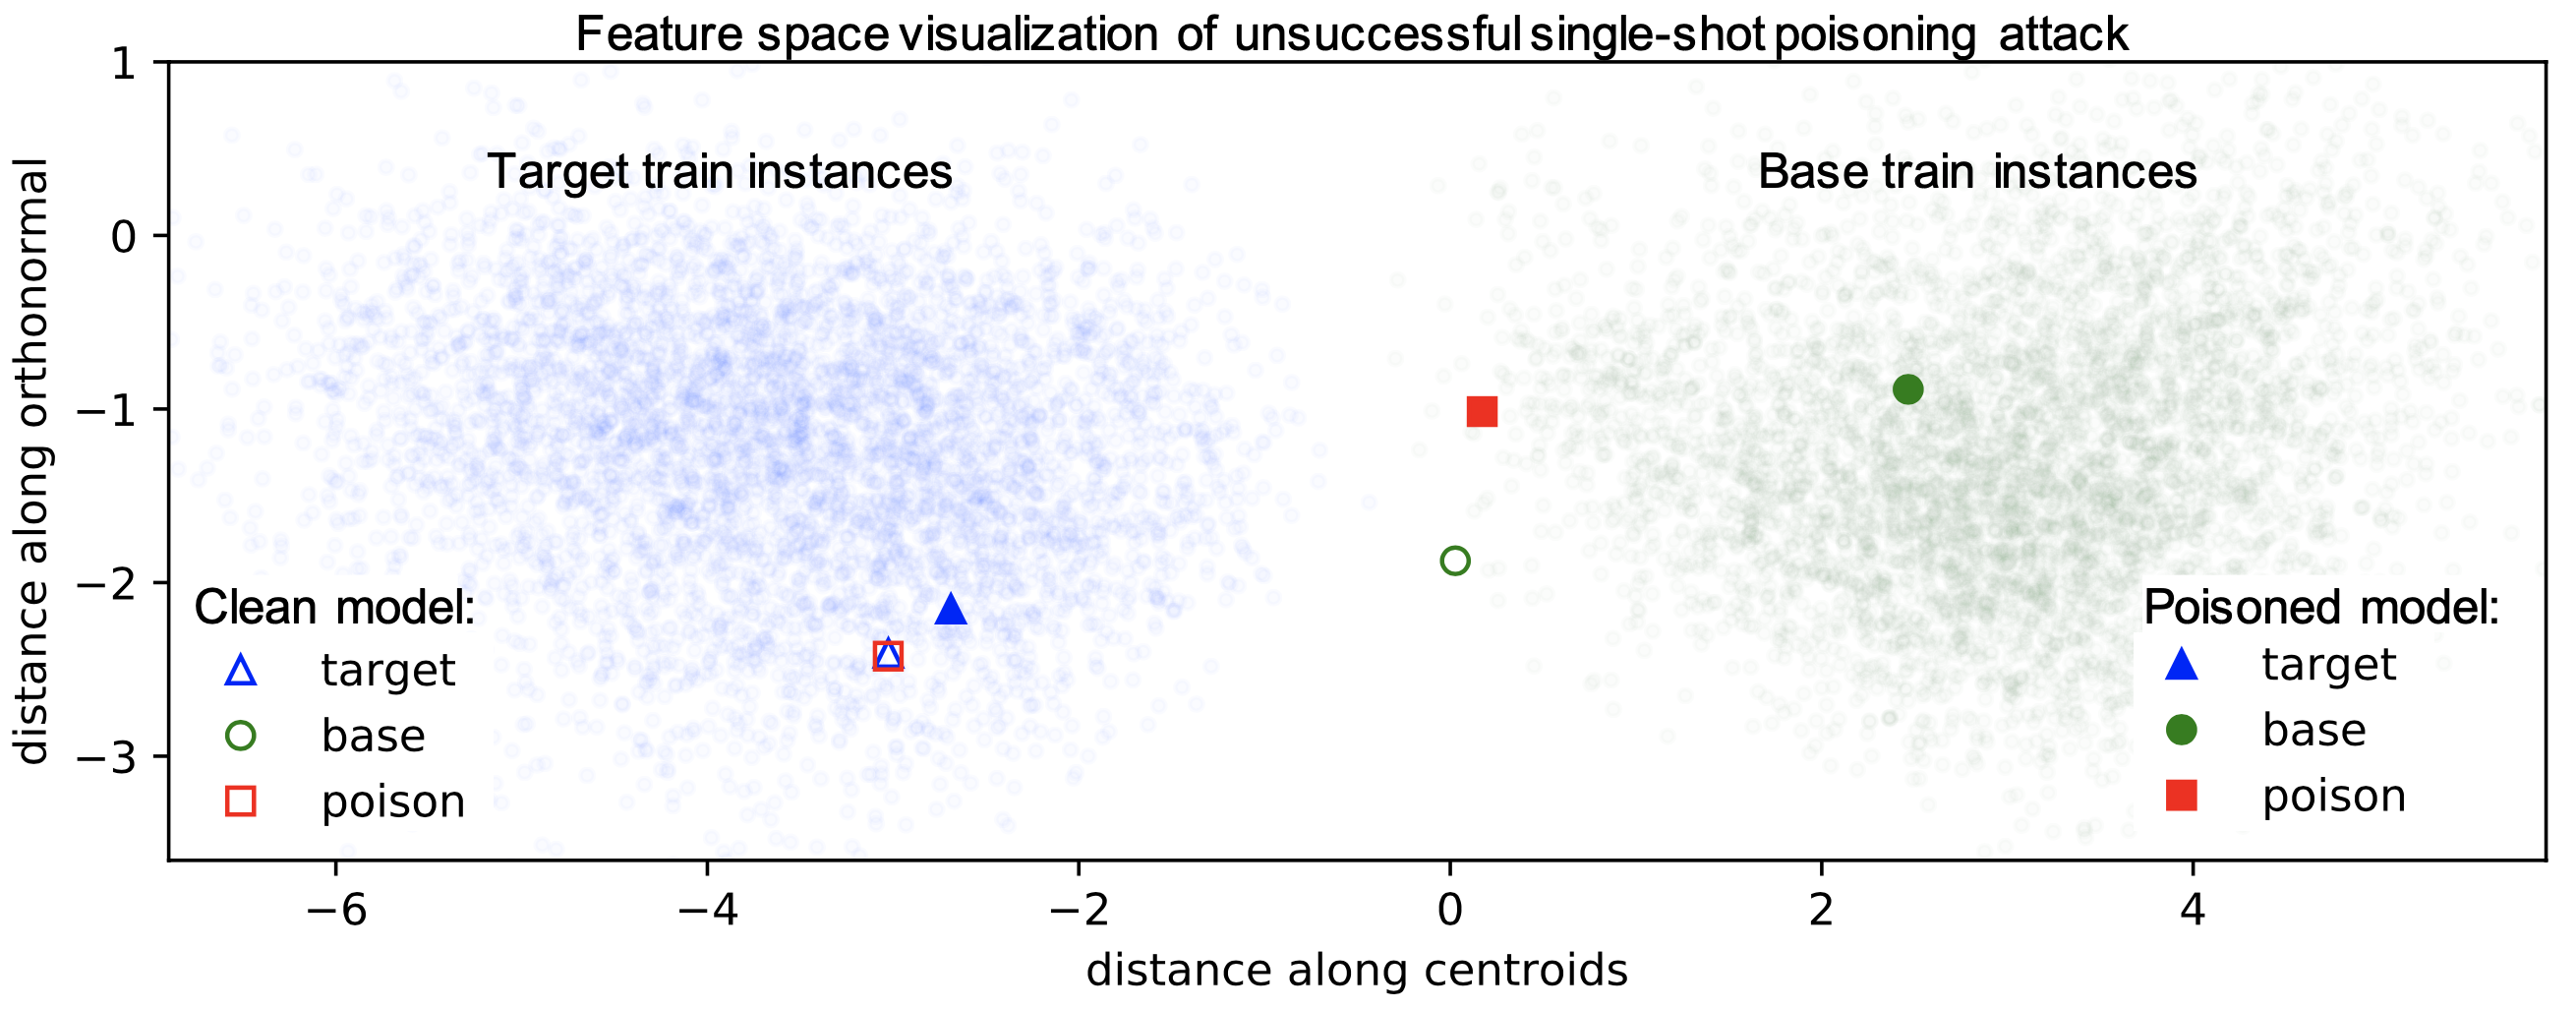
\includegraphics[width=15cm]{figures/end2end_distribute.png}
	\caption{One shot kill attacks do not work, multiple poisons are required. \color{red}{Feature layers learn to separate poison from target in feature space.}}
	\label{fig:end2end_distribute}
\end{figure}

\begin{figure}[!h]
	\centering
	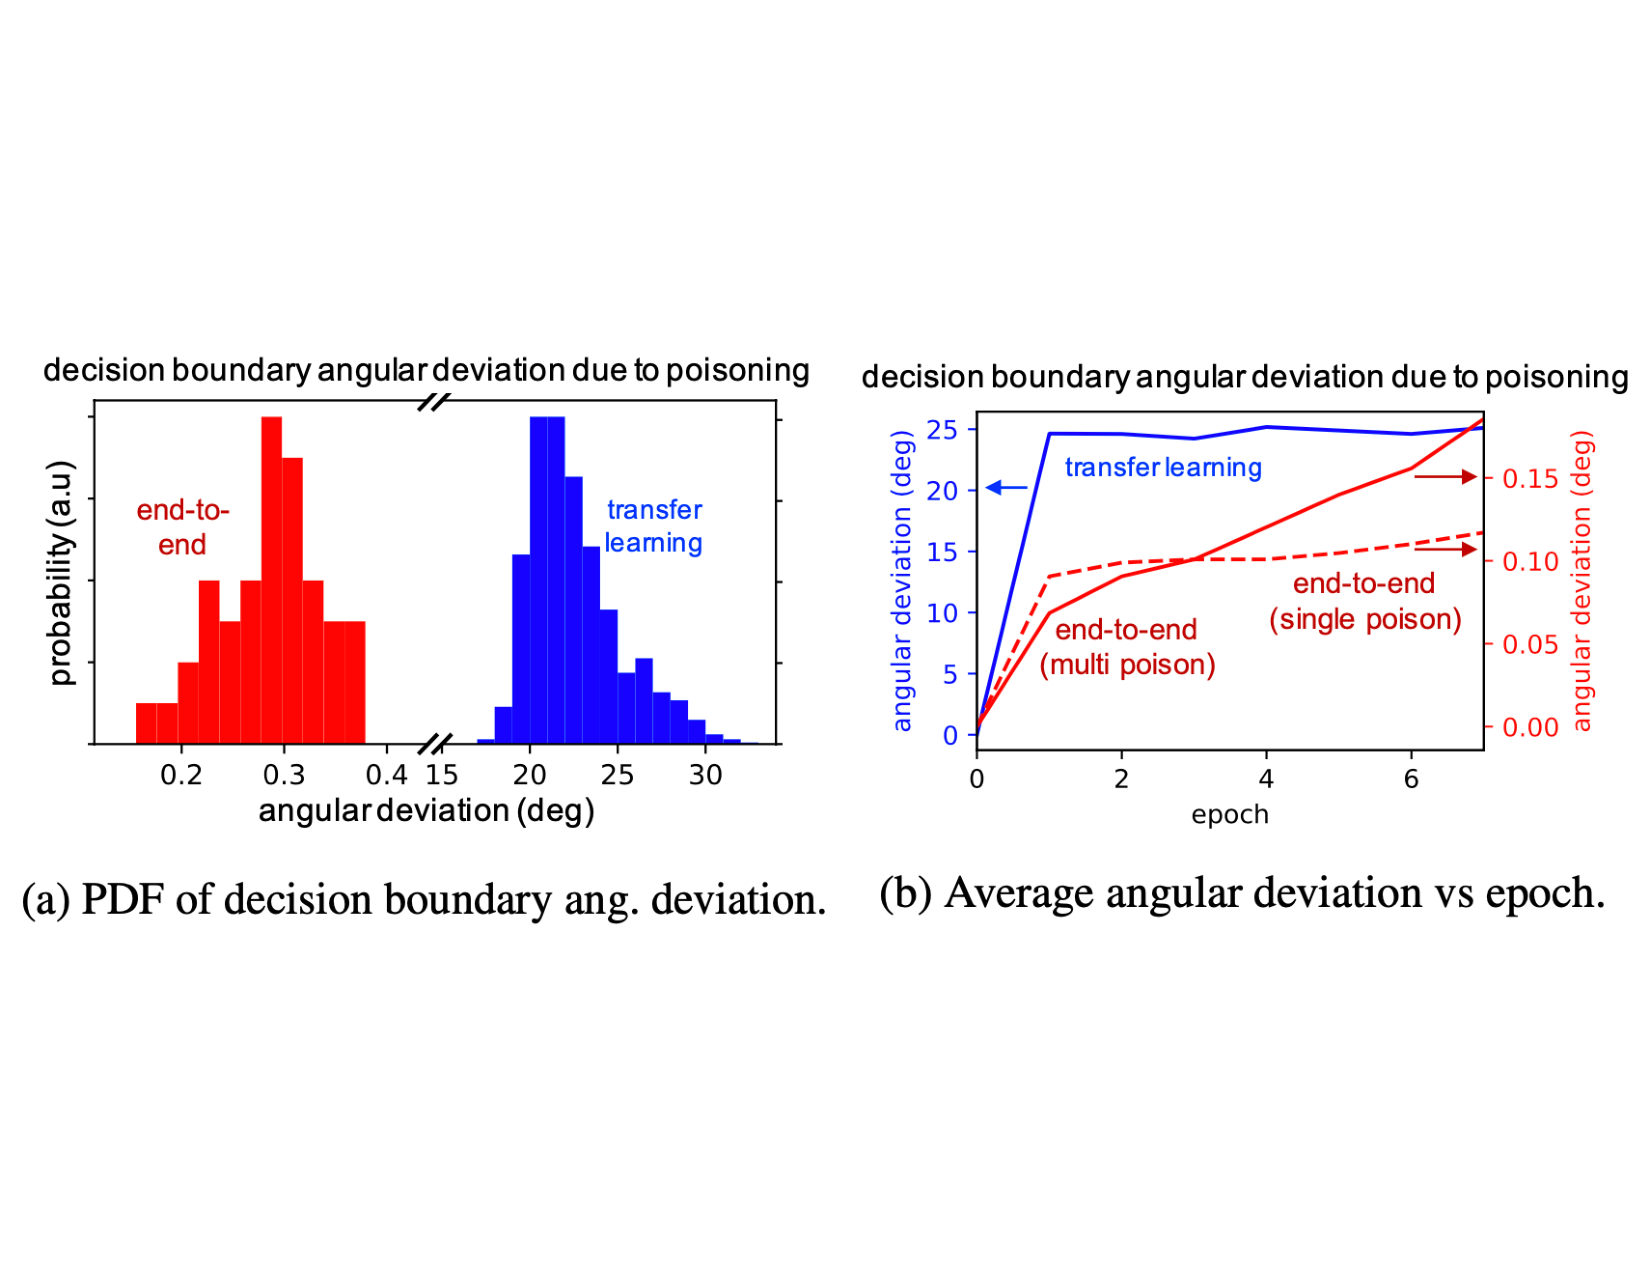
\includegraphics[width=14cm]{figures/Angular.pdf}
	\caption{Angular deviation of the feature space decision boundary}
	\label{fig:P_misclassify}
\end{figure}

In transfer learning, there is a significant rotation (average of 23 degrees) in the feature space decision boundary. For the end-to-end training experiments, the decision boundary barely changes.

Fooling the feature extractors require:
\begin{itemize}
    \item Watermarking: overlay the target onto the poison\\
    A base watermarked image with target opacity $\gamma$:
    \begin{equation*}
        \bb \leftarrow \gamma \cdot \t + (1 - \gamma) \cdot \bb
    \end{equation*}

    \item Using multiple Poisons
\end{itemize}

\begin{figure}[H]
  \centering 
  \subfigure[Watermarking]{ 
    \centering
    \label{fig:subfig:a} %% label for first subfigure 
    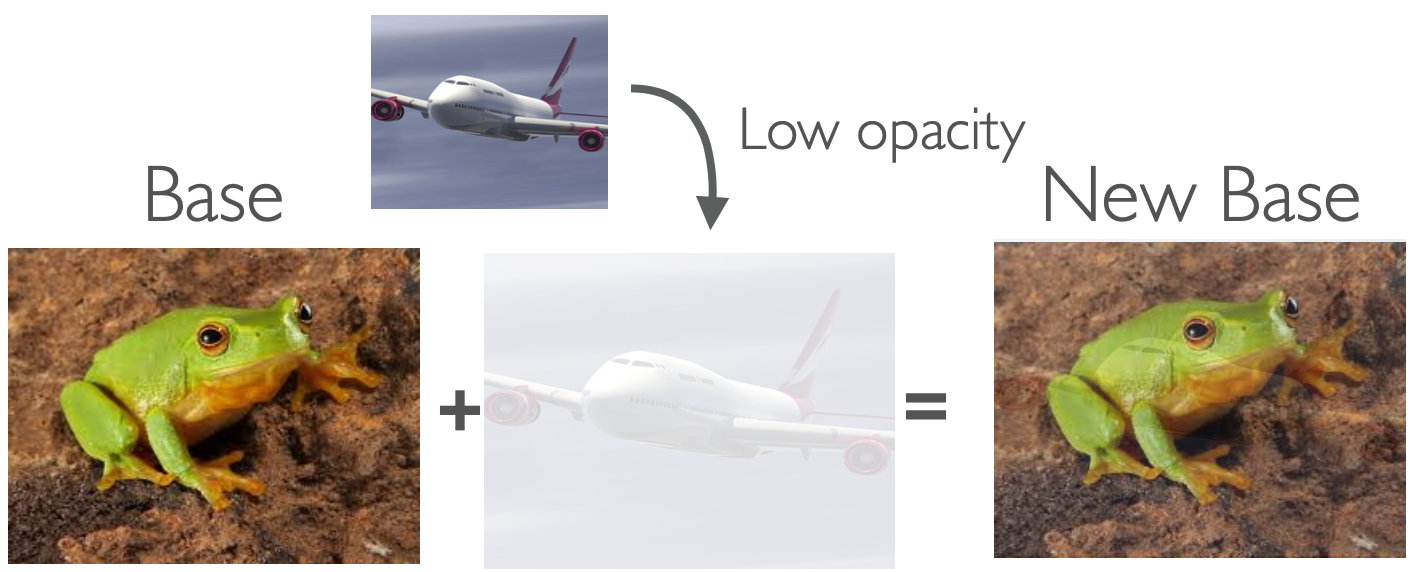
\includegraphics[width=8cm]{figures/watermark.png}} 
  \hspace{0.3cm} 
  \subfigure[multiple poisons]{ 
    \centering
    \label{fig:subfig:b} %% label for second subfigure 
    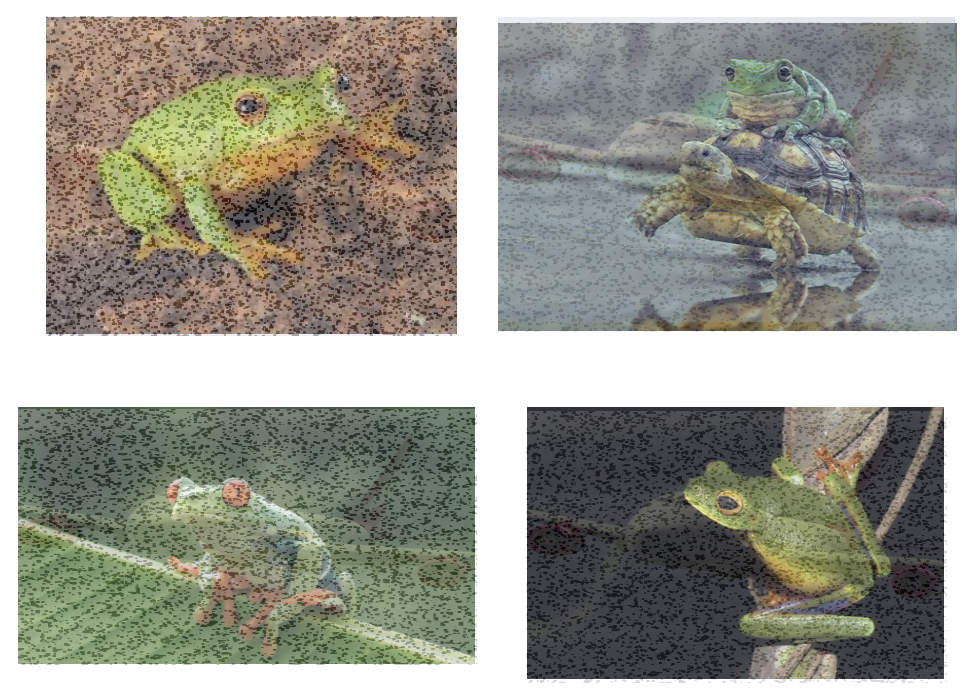
\includegraphics[width=6cm]{figures/multiple_poisons.png}} 
%   \caption{Two Subfigures} 
  \label{fig:end2end_require} %% label for entire figure 
\end{figure}

\begin{figure}[!h]
	\centering
	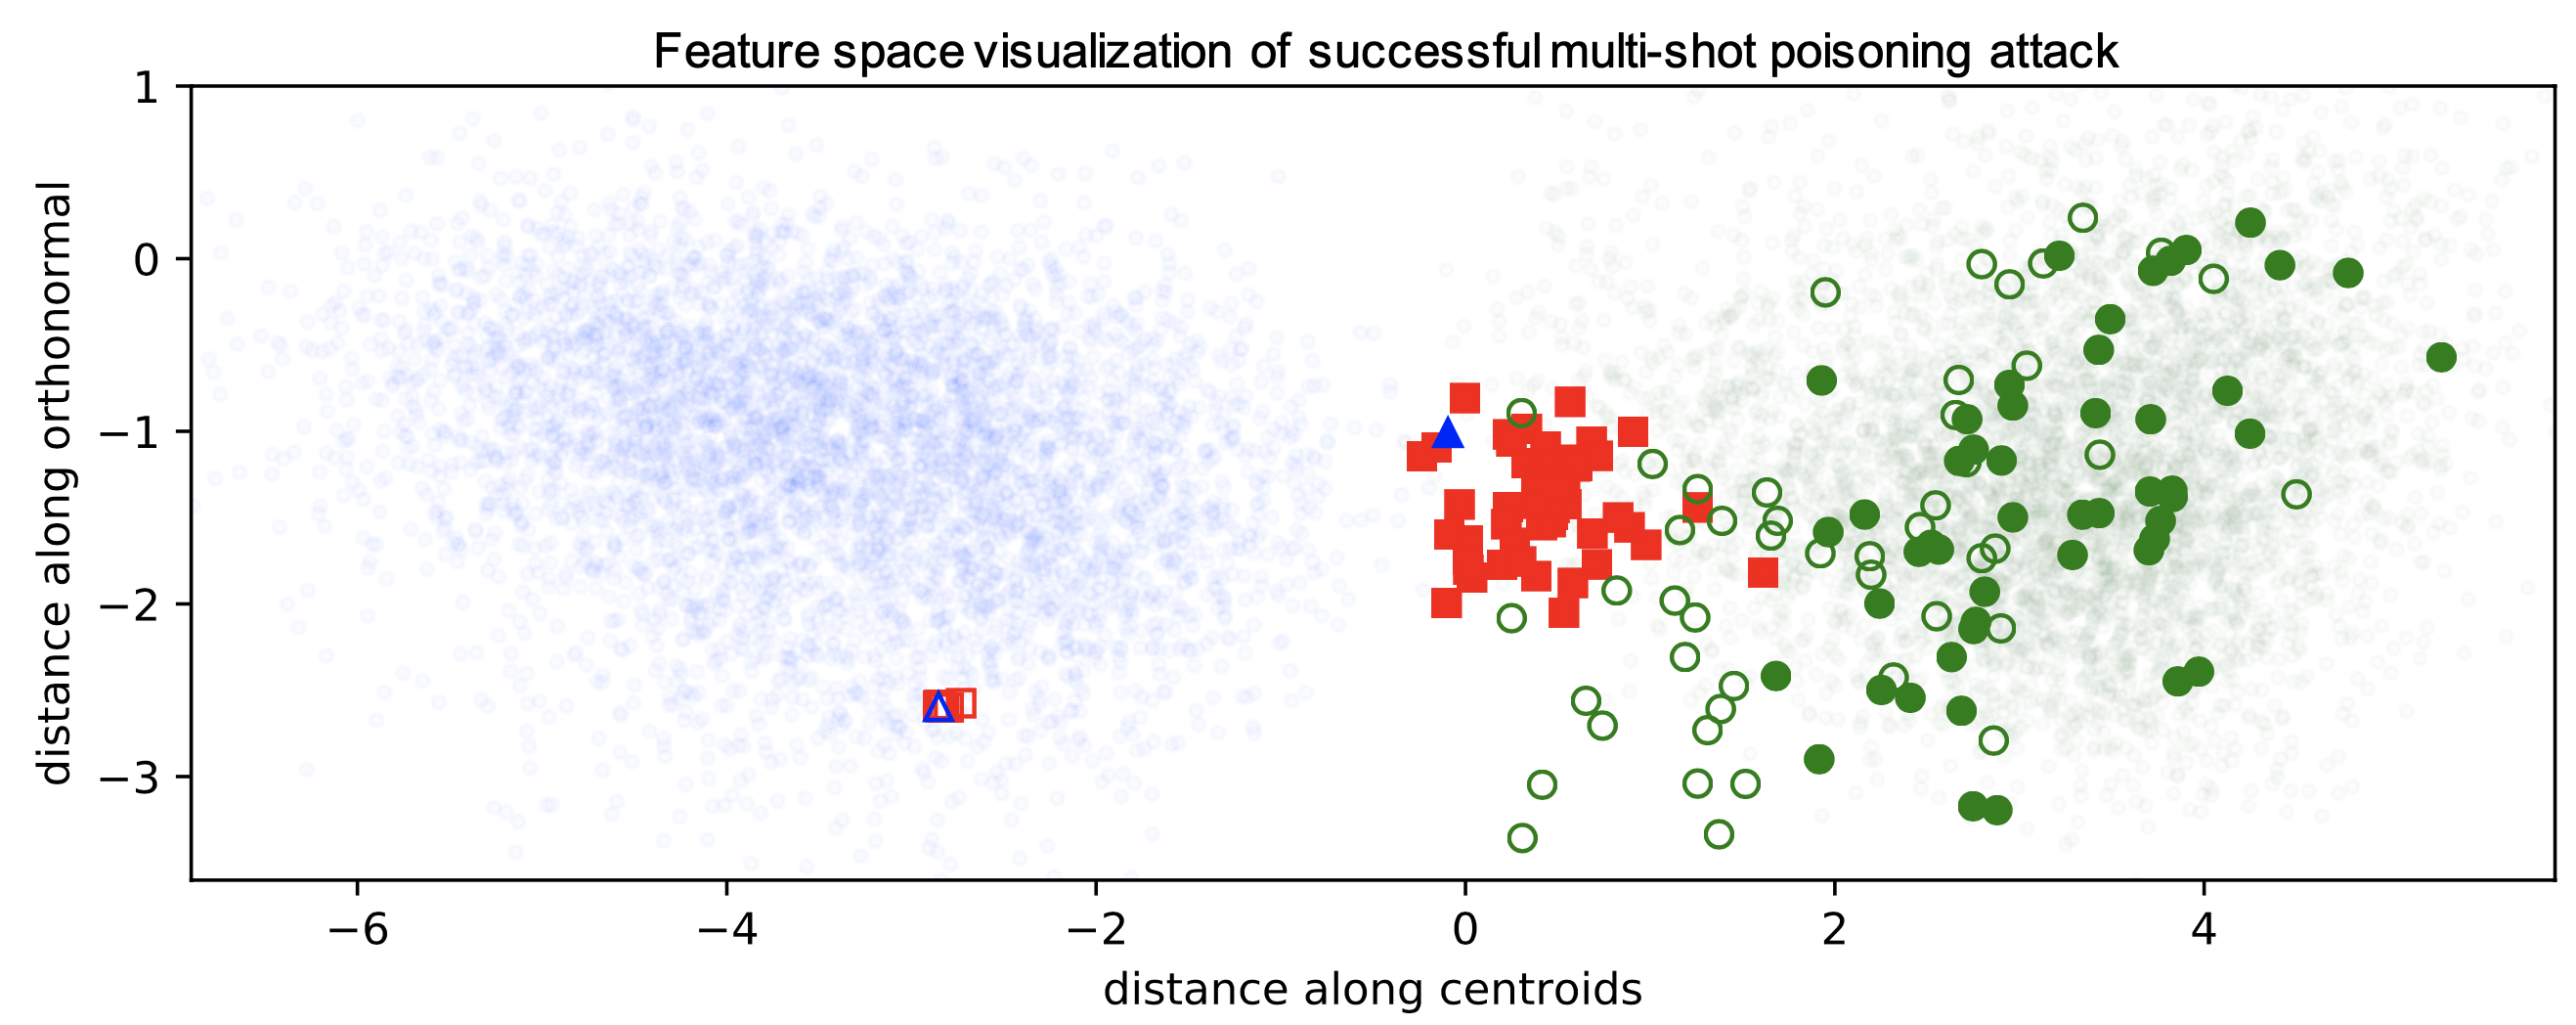
\includegraphics[width=14cm]{figures/end2end_both.png}
	\caption{Target instance is pulled out of the target class distribution (in feature space) into the base class distribution and get incorrectly classified as the base class.}
	\label{fig:end2end_both}
\end{figure}

\begin{figure}[!h]
	\centering
	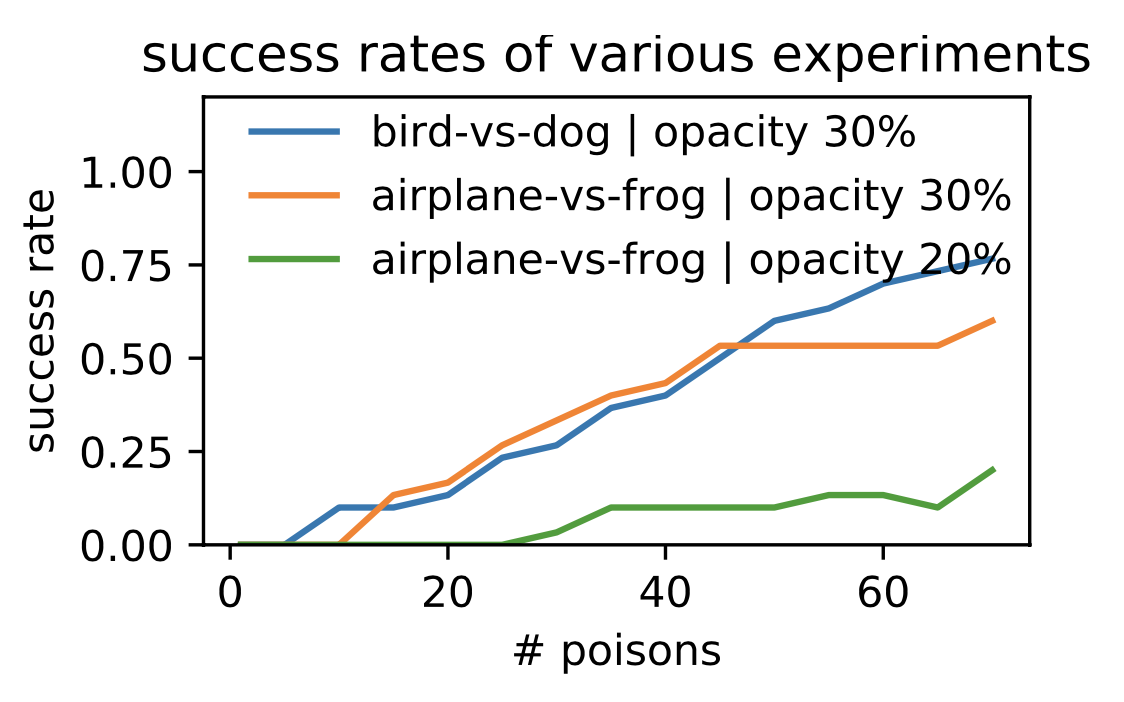
\includegraphics[width=10cm]{figures/end2end_successful_rate.png}
	\caption{Success rate of attacks on different targets from different bases as a function of number of poison instances used and different target opacity added to the base instances.}
% 	\label{fig:end2end_both}
\end{figure}


% \subsection{Basic Idea}

% Recall that the bottleneck of AGD is at the computation of $\g (\w)$.
% The data partition can be formally captured by the $m$ disjoint sets: $\SM_1, \cdots , \SM_m$;
% if the sample $(\x_j, y_j)$ is in the $k$-th worker node, then $j \in \SM_k$.
% The gradient $\g (\w)$ in \eqref{eq:grad_sum} can be rewritten as
% \begin{eqnarray} \label{eq:grad1}
%     \g (\w ) 
%     & = & \frac{1}{n} \sum_{k=1}^m 
%     \underbrace{\sum_{j \in \SM_k} \frac{ \partial \, L (\w; \x_j, y_j) }{ \partial \, \w } }_{ \tilde{\g}_k (\w ) } 
%     + \frac{ \partial \, R (\w) }{ \partial \, \w }  .
% \end{eqnarray}
% Note that $\tilde{\g}_k (\w) \in \RB^d$ depends only on $\w$ and the $k$-th worker's data.
% Thus, upon receiving $\w$, the $k$-th worker is able to compute $\tilde{\g} (\w)$.
% We can equivalently write \eqref{eq:grad1} as
% \begin{eqnarray} \label{eq:grad2}
%     \g (\w ) 
%     & = & \frac{1}{n} \sum_{k=1}^m  \tilde{\g}_k (\w )  + \frac{ \partial \, R (\w) }{ \partial \, \w } .
% \end{eqnarray}
% Note also that $\frac{ \partial \, R (\w) }{ \partial \, \w }$ depends only on $\w$, and thus the server can compute it locally.
% The server aggregates $\tilde{\g}_1 (\w), \cdots ,  \tilde{\g}_m (\w)$ and then compute $\g (\w)$ according to \eqref{eq:grad2}.







% \subsection{Algorithm Description} \label{sec:pagd:alg}

% The AGD algorithm developed in Section~\ref{sec:optimization} can be implemented in the following way to fit the parallel computing framework.
% Parallel AGD repeats the following four steps till convergence.

% \paragraph{Broadcast.}
% The central parameter server stores the latest model parameters, say $\w_t \in \RB^d$.
% The server {broadcasts} $\w_t$ to the workers so that the workers will have the latest parameters.
% The time complexity of this step is negligible; the communication complexity is $\OM (d m)$ words.
% (By organizing the workers nodes as a binary tree, the communication cost can be $\OM (d \log m)$.)


% \paragraph{Workers' local computation.}
% Upon receiving $\w_t$, the $k$-th worker uses its local data (which are indexed by $\SM_k$) to compute the \textit{local gradient} $\tilde{\g}_k (\w_t )$:
% \begin{equation} \label{eq:grad3}
%     \tilde{\g}_k (\w_t ) \: = \: \sum_{j \in \SM_k} \frac{ \partial \, L (\w; \x_j, y_j) }{ \partial \, \w } \bigg|_{\w = \w_t} .
% \end{equation}
% This step does not need communication.
% For least squares and logistic regression, the time complexity is $\OM (d \, |\SM_k |)$.


% \paragraph{Aggregate the local gradients.}
% The workers send their local gradients, $\tilde{\g}_1 (\w_t), \cdots , \tilde{\g}_m (\w_t)$ to the server.
% The server aggregates the local gradients by $\frac{1}{n} \sum_{k=1}^m  \tilde{\g}_k (\w_t ) $ and then compute the gradient $\g (\w_t )$ according to \eqref{eq:grad2}.
% The server needs to compute the differential $\frac{\partial \, R (\w) }{\partial \, \w} \big|_{\w = \w_t }$ and sum the local gradients, which are inexpensive operations.
% The aggregation requires all-to-one communication of the local gradients which has $\OM (d m )$ or $\OM (d \log m)$ time complexity, depending on the computer network structure.


% \paragraph{Server updates the model parameters.}
% With $\g (\w_t )$ at hand, the server updates the momentum by $\v_{t+1} = \beta \v_t + \g (\w_t )$ and the model parameters by $\w_{t+1} = \w_t - \alpha \v_{t+1}$.
% This step does not have communication.
% These operations have merely $\OM (d)$ time complexity. 



% \subsection{Analyzing the Costs}

% \paragraph{Computational costs.}
% As aforementioned, the computation of AGD is mostly in computing the gradient.
% In parallel AGD, the gradient is computated by $m$ workers in parallel.
% If the work load is balanced, then every worker has a per-iteration time complexity of $\OM (n d / m)$.
% The server performs inexpensive vector operations, and its computational cost is negligible.



% \paragraph{Communication costs.}
% Every iteration of the parallel AGD algorithm has two communications: one-to-all broadcast and all-to-one aggregation.
% The communication complexities is $\OM (d m)$ words if the connections between the server and workers form a ``star graph'';
% it is $\OM (d \log m)$ if the network connection is a binary tree structure.


% What is the time cost of one communication?
% It mainly depends on the bandwidth (denote $B$) and latency\footnote{When the server sends a message to a worker, the work does not receive the message immediately, even if the package has only one bit. Network latency is an expression of how much time it takes for a packet of data to get from one designated point to another.} (denote $L$) of the network and the communication complexity (denote $C$) of the algorithm.
% Then the time cost is approximately $\frac{C}{B} + L$.



% \paragraph{Synchronization costs.}
% This algorithm is bulk synchronous, the server will wait for all the workers to complete before starting the next iteration.
% An obvious shortcoming is that everyone must wait for the slowest worker to complete; see the illustration in Figure~\ref{fig:synchronization}.
% If a worker fails (due to hardware or software failure) and restarts, then the time cost of this iteration will double.
% This worker is called straggler, and this phenomenon is known as the {straggler effect}.
% It is exacerbated as the number of workers increases.
% If a worker fails with probability $1\%$ and there are 50 workers, then with probability $60\%$, there will be at least one node fail.
% Asynchronous algorithms, e.g., \cite{recht2011hogwild}, are typically faster than the synchronous.



% \begin{figure}[!h]
% 	\centering
% 	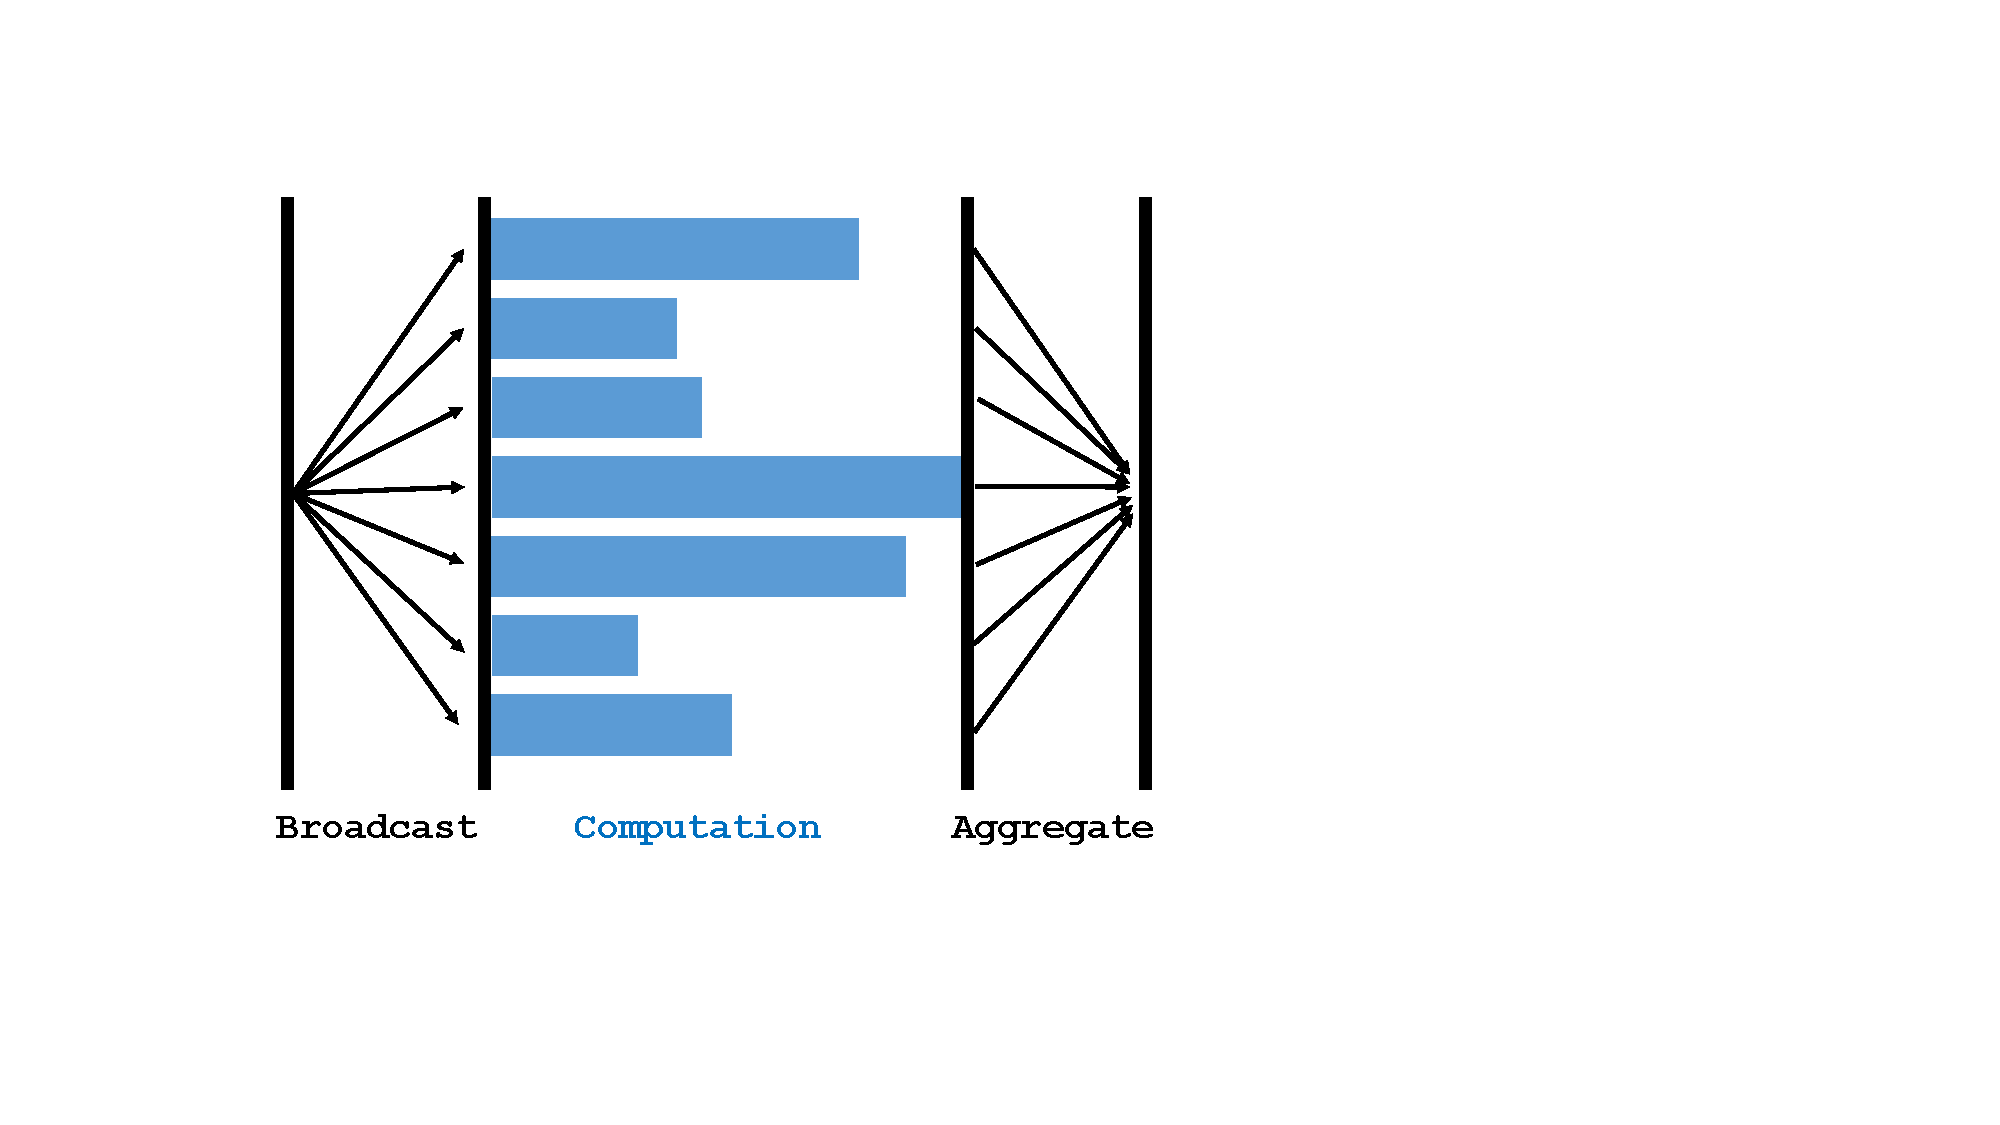
\includegraphics[width=0.6\linewidth]{figures/Communication.pdf}
% 	\caption{Illustration of synchronization.}
% 	\label{fig:synchronization}
% \end{figure}


% \paragraph{Speedup ratio.}
% Ideally, since the computation of gradient is performed by $m$ workers in parallel, the wall-clock runtime can be $\frac{1}{m}$ of the single-machine AGD.
% If it is the case, then we say the speedup ratio is $m$.
% Unfortunately, due to the other overhead, the speedup ratio is always smaller than $m$; when $m$ is large, the growth rate of speedup ratio is slow.
% See Figure~\ref{fig:speedup} for the illustration.


% \begin{figure}[!h]
% 	\centering
% 	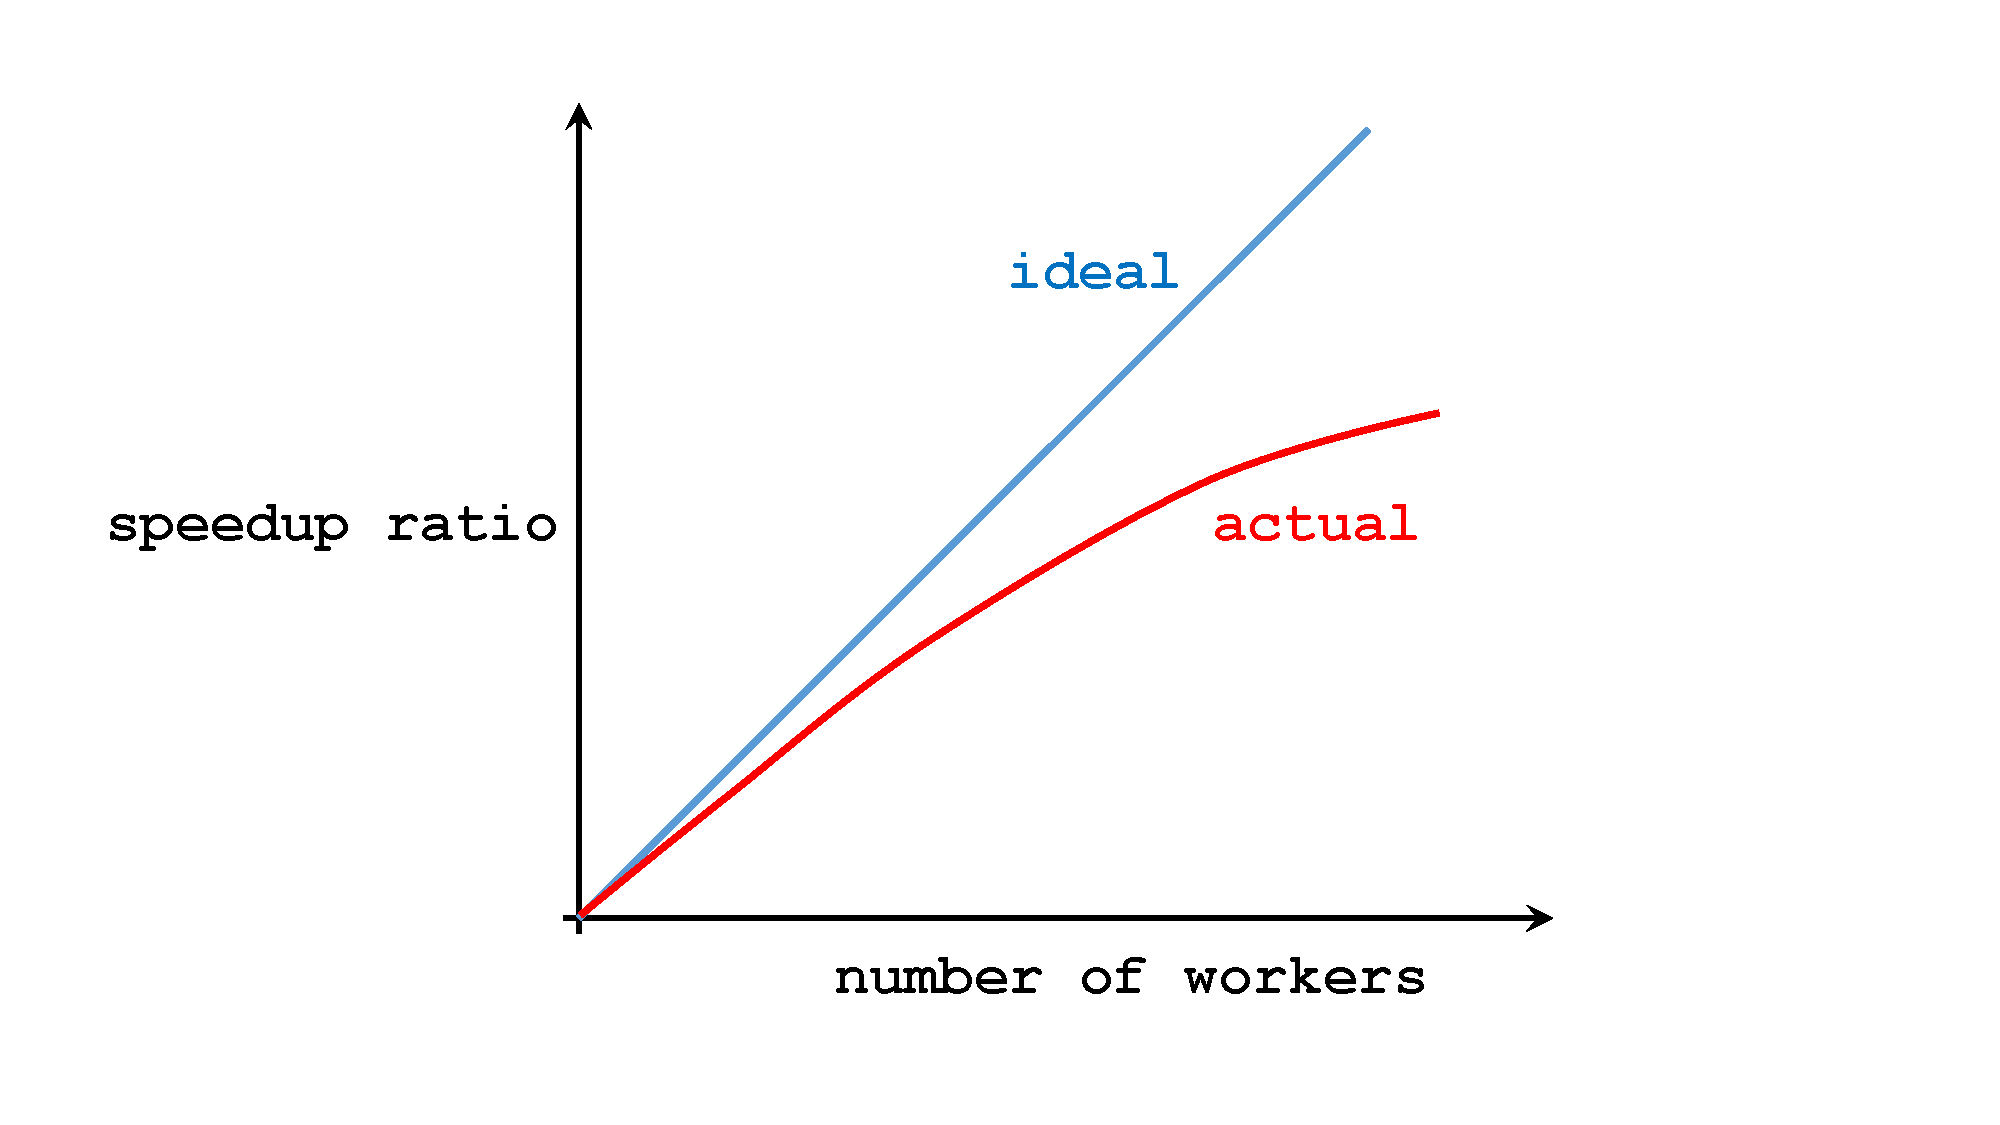
\includegraphics[width=0.6\linewidth]{figures/speedup.pdf}
% 	\caption{Ideal and actual speedup ratios.}
% 	\label{fig:speedup}
% \end{figure}


% \section{Python Implementation for Logistic Regression}


% Let us implement a simulator that mimics synchronous parallel AGD for the $\ell_2$-norm regularized logistic regression:
% \begin{equation} \label{eq:model}
% \min_{\w \in \RB^d} \;
% \Bigg\{  
% Q (\w ; \X , \y ) \: \triangleq \:
% \frac{1}{n}  \sum_{j=1}^n \log \Big( 1 + \exp \big( - y_j \x_j^T \w\big) \Big) 
% \, + \, \frac{\lambda}{2} \, \| \w \|_2^2 \Bigg\} .
% \end{equation}
% Our code does not actually perform parallel computing, but it will help the reader understand how parallel AGD works.
% To actually make use of multiple processors, the reader needs to learn Message Passing Interface (MPI), Apache Spark \cite{zaharia2010spark}, Ray \cite{moritz2018ray}, or other software system.



% \subsection{Worker Node}

% A worker node receives a partition of data in the beginning and holds the data throughout.
% Let $\SM$ ($|\SM | = s$) index the samples held by this worker.
% Its \textsf{loss()} function computes the local loss
% \begin{equation*}
%     \tilde{L} (\w) \: = \: 
%     \sum_{j \in \SM} \log \big( 1 + \exp (-y_j \x_j^T \w ) \big) .
% \end{equation*}
% Its \textsf{gradient()} function the local gradient
% \begin{equation*}
%     \tilde{\g} (\w ) \: = \:
%     \sum_{j \in \SM} \frac{ - y_j \x_j }{1+\exp({y_j \w^T \x_j})} .
% \end{equation*}

% \vspace{3mm}
% \begin{lstlisting}
% class Worker:
%     def __init__(self, x, y):
%         self.x = x # s-by-d local feature matrix
%         self.y = y # s-by-1 local label matrix
%         self.s = x.shape[0] # number of local samples
%         self.d = x.shape[1] # number of features
%         self.w = numpy.zeros((d, 1)) # d-by-1 model parameter vector
        
%     # Set the model parameters to the latest
%     def set_param(self, w):
%         self.w = w
    
%     # Compute the local loss 
%     def loss(self):
%         yx = numpy.multiply(self.y, self.x) # s-by-d matrix
%         yxw = numpy.dot(yx, self.w) # s-by-1 matrix
%         vec1 = numpy.exp(-yxw) # s-by-1 matrix
%         vec2 = numpy.log(1 + vec1) # s-by-1 matrix
%         return numpy.sum(vec2) # loss function
    
%     # Compute the local gradient
%     def gradient(self):
%         yx = numpy.multiply(self.y, self.x) # s-by-d matrix
%         yxw = numpy.dot(yx, self.w) # s-by-1 matrix
%         vec1 = numpy.exp(yxw) # s-by-1 matrix
%         vec2 = numpy.divide(yx, 1+vec1) # s-by-d matrix
%         g = -numpy.sum(vec2, axis=0).reshape(self.d, 1) # d-by-1 matrix
%         return g
% \end{lstlisting}
% \vspace{3mm}




% \subsection{Server}

% The server maintains and updates the model parameters; it does not store the data samples.
% In the \textsf{init()} function, we let the server know that there are $m$ workers, $n$ training samples, and $d$ features.
% After the workers complete computing the local losses $\tilde{L}_{1} (\w) , \cdots , \tilde{L}_m (\w)$ and gradients $\tilde{\g}_{1} (\w) , \cdots , \tilde{\g}_m (\w)$, the server's \textsf{aggregate()} function computes 
% \begin{equation*}
%     \sum_{k=1}^m \tilde{\g}_{k} (\w) 
%     \qquad \textrm{and} \qquad
%     \sum_{k=1}^m \tilde{L}_{k} (\w).
% \end{equation*}
% The \textsf{gradient()} function computes the full gradient
% \begin{equation*}
%     \g (\w )
%     \: = \: \frac{1}{n} \sum_{k=1}^m \tilde{\g}_{k} (\w) + \lambda \w .
% \end{equation*}
% The \textsf{objective()} function computes
% \begin{equation*}
%     Q (\w ; \X , \y)
%     \: = \: \frac{1}{n} \sum_{k=1}^m \tilde{L}_{k} (\w) + \frac{\lambda }{2 } \| \w \|_2^2 ,
% \end{equation*}
% which helps monitor the progress of the optimization.
% The \textsf{agd()} function updates momentum and then the model parameters by
% \begin{equation*}
%     \v \longleftarrow \beta \v + \g (\w) 
%     \qquad \textrm{and} \qquad
%     \w \longleftarrow \w - \alpha \v ,
% \end{equation*}
% which completes an iteration.

% \vspace{3mm}
% \begin{lstlisting}
% class Server:
%     def __init__(self, m, n, d):
%         self.m = m # number of worker nodes
%         self.n = n # number of training samples
%         self.d = d # number of features
%         self.w = numpy.zeros((d, 1)) # # d-by-1 model parameter vector
%         self.g = numpy.zeros((d, 1)) # d-by-1 gradient
%         self.v = numpy.zeros((d, 1)) # d-by-1 momentum
%         self.loss = 0 # loss function value
%         self.obj = 0 # objective function value
            
%     def broadcast(self):
%         return self.w
            
%     # Sum the gradients and loss functions evaluated by the workers
%     # Args:
%     #   grads: a list of d-by-1 vectors
%     #   losses: a list of scalars
%     def aggregate(self, grads, losses):
%         self.g = numpy.zeros((self.d, 1))
%         self.loss = 0
%         for k in range(self.m):
%             self.g += grads[k]
%             self.loss += losses[k]
    
%     # Compute the gradient (from the loss and regularization)
%     def gradient(self, lam):
%         self.g = self.g / self.n + lam * self.w        
        
%     # Compute the objective function (sum of loss and regularization)
%     def objective(self, lam):
%         reg = lam / 2 * numpy.sum(self.w * self.w) 
%         self.obj = self.loss / self.n + reg
%         return self.obj
    
%     # Update the model parameters using accelerated gradient descent
%     # Args:
%     #   alpha: learning rate (step size)
%     #   beta: momentum parameter
%     def agd(self, alpha, beta):
%         self.v *= beta
%         self.v += self.g
%         self.w -= alpha * self.v
% \end{lstlisting}
% \vspace{3mm}


% \subsection{Initialization}

% The following function create one server and a list of $m$ workers.
% We are given $n$ samples which are stored in $\X \in \RB^{n\times d}$ and $\y \in\RB^n$.
% We partition the $n$ samples to $m$ parts and use each part to create one worker.


% \vspace{3mm}
% \begin{lstlisting}
% import math

% # Create a server and m worker nodes
% def create_server_workers(m, x, y):
%     n, d = x.shape
%     s = math.floor(n / m)
%     server = Server(m, n, d)
%     workers = []

%     for i in range(m): 
%         indices = list(range(i*s, (i+1)*s))
%         worker = Worker(x[indices, :], y[indices, :])
%         workers.append(worker)
        
%     return server, workers
% \end{lstlisting}
% \vspace{3mm}


% We use $m=4$ workers and apply the function \textsf{create\_server\_workers}.
% The returned are \textsf{server} (an object) and \textsf{workers} (a list of objects).

% \vspace{3mm}
% \begin{lstlisting}
% m = 4 # number of worker nodes
% server, workers = create_server_workers(m, x_train, y_train)
% \end{lstlisting}
% \vspace{3mm}


% \begin{figure}[!h]
% 	\centering
% 	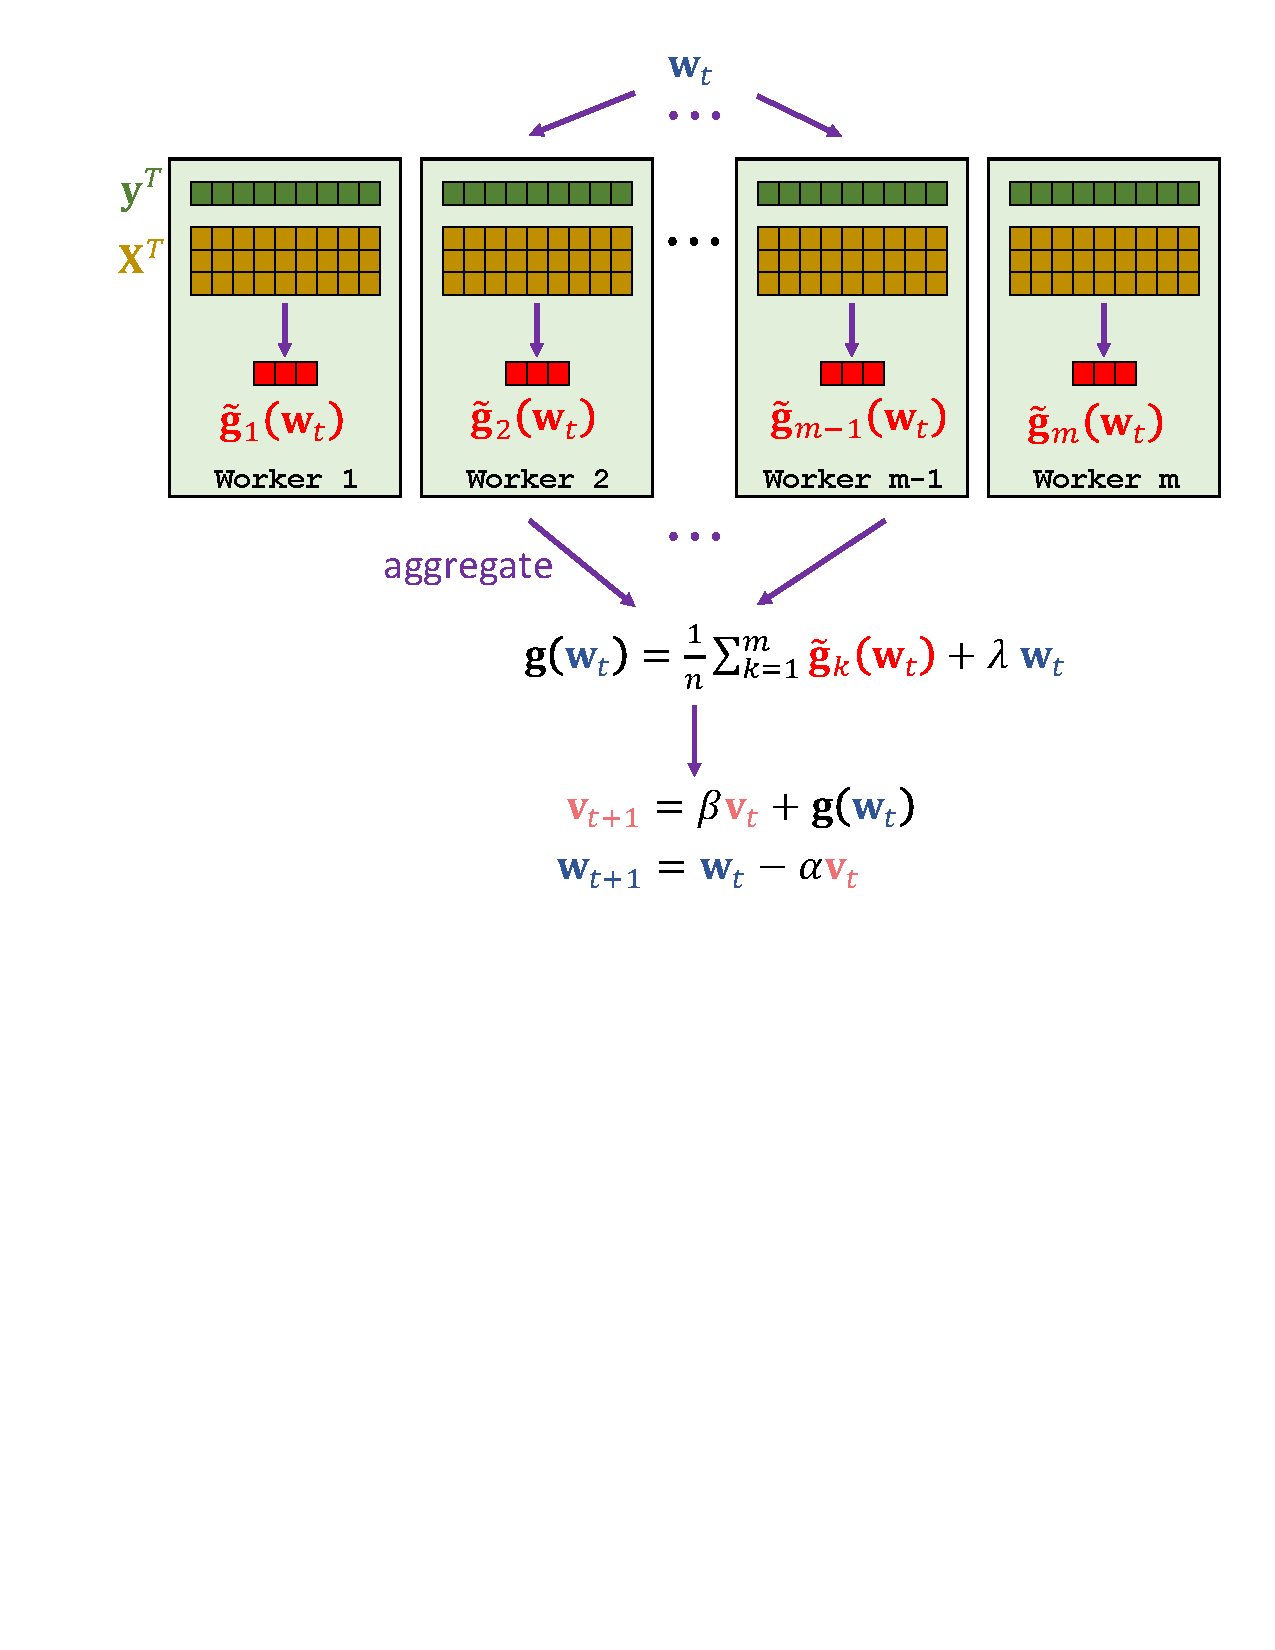
\includegraphics[width=0.6\linewidth]{figures/AGD.pdf}
% 	\caption{Illustration of parallel AGD.}
% 	\label{fig:agd}
% \end{figure}

% \subsection{Performing Parallel AGD}

% With the server and workers set up, we are ready to run the parallel AGD algorithm.
% The following code executes the parallel AGD algorithm described in Section~\ref{sec:pagd:alg}.
% We illustrate the procedure in Figure~\ref{fig:agd}




% \vspace{3mm}
% \begin{lstlisting}
% lam = 1E-6 # regularization parameter
% alpha = 1E-1 # learning rate
% beta = 0.9 # momentum parameter
% max_epoch = 50 # number of epochs

% for t in range(max_epoch):
%     # step 1: broadcast
%     w = server.broadcast()
%     for i in range(m):
%         workers[i].set_param(w)
        
%     # step 2: workers' local computations
%     grads = []
%     losses = []
%     for i in range(m):
%         g = workers[i].gradient()
%         grads.append(g)
%         l = workers[i].loss()
%         losses.append(l)
        
%     # step 3: aggregate the workers' outputs
%     server.aggregate(grads, losses)
    
%     # step 4: server update the model parameters
%     server.gradient(lam) # compute gradient
%     obj = server.objective(lam) # compute compute objective function
%     print('Objective function value = ' + str(obj))
%     server.agd(alpha, beta) # updates the model parameters
% \end{lstlisting}
% \vspace{3mm}



% \section{Problems}

% The readers are encouraged to write simulators for the following algorithms.

% \subsection{Federated Averaging}

% Federated Averaging (\textsf{FedAvg}) \citep{mcmahan2017communication} is similar to the parallel gradient descent (GD): 
% \textsf{FedAvg} has a central parameter server, the data are partitioned among the worker nodes, and it is synchronous.
% Instead of performing one GD or stochastic gradient descent (SGD), every worker locally run multiple GDs (or SGDs) and return the descending direction to the server.
% In this way, every worker performs more computation, but the overall communication is reduced.
% If communication is the bottleneck, then \textsf{FedAvg} is more practical than parallel GD.

% Here we briefly describe the algorithm.
% \textsf{FedAvg} repeats the following steps till convergence.
% \begin{itemize}
%     \item 
%     The server broadcasts $\w$ to all the workers.
%     \item
%     Upon receiving $\w$, a worker (say the $k$-th) uses its local data to locally performs $q$ ($\geq 1$) GDs (or SGDs).
%     Let $\tilde{\w}_{k}$ be the result of the $q$ local GDs (or SGDs).
%     The the ascending direction computed by the $k$-th worker is
%     \begin{equation*}
%         \tilde{\pp}_{k} \: = \: \w - \tilde{\w}_{k}  .
%     \end{equation*}
%     \item
%     The server aggregates $\tilde{\pp}_{1}, \cdots , \tilde{\pp}_{m}$:
%     \begin{equation*}
%         \pp \: = \: \frac{1}{m} \sum_{k=1}^m \tilde{\pp}_{k} .
%     \end{equation*}
%     The server then update the model parameters by
%     \begin{equation*}
%         \w \: \longleftarrow \: \w - \alpha \pp 
%     \end{equation*}
%     and decrease the learning rate $\alpha$.
% \end{itemize}
% In the case of $q = 1$, \textsf{FedAvg} is the same to parallel GD (or SGD).


% \subsection{Decentralized Optimization}

% Decentralized optimization allows for worker nodes jointly learn a model without have a central server.
% Every worker is connected to some other workers; see the illustration in Figure~\ref{fig:decentralized}.
% Many decentralized algorithms have been developed for solving this problem~\cite{bianchi2013performance,yuan2016convergence,sirb2016consensus,colin2016gossip,lian2017can,lan2017communication,tang2018d}. 
% A typical decentralized algorithms~\cite{lian2017can} works in this way:
% a node collects its neighbors' model parameters, weighted averages its neighbors' and its own parameters, and performs an (stochastic) gradient descent to update its local parameters.



% \begin{figure}[!h]
% 	\centering
% 	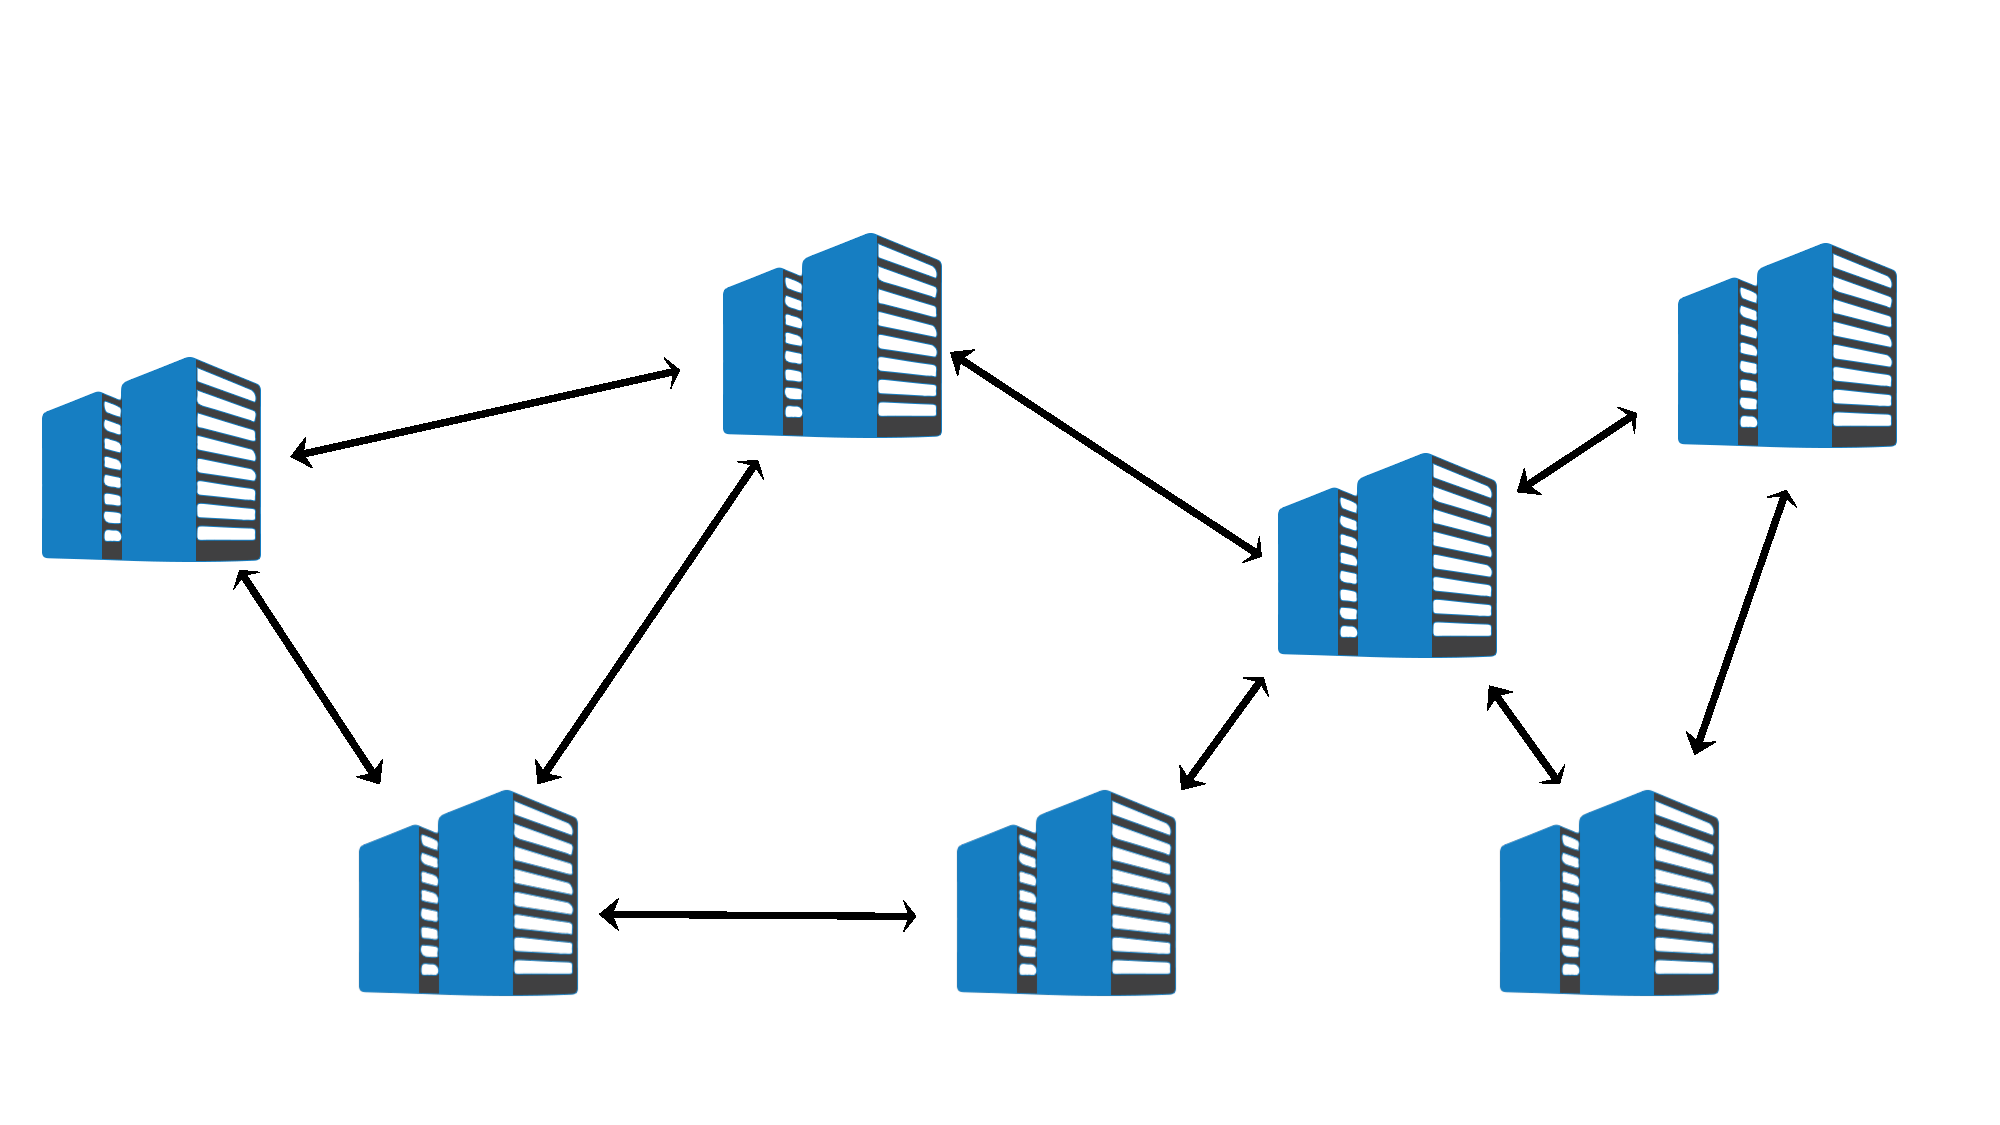
\includegraphics[width=0.6\linewidth]{figures/decentralized.pdf}
% 	\caption{Illustration of a decentralized system.}
% 	\label{fig:decentralized}
% \end{figure}


% \paragraph{Hints for implementation.}
% (1). You can use a set of seven workers connected in the way of Figure~\ref{fig:decentralized}.
% (2). Every worker node has a list of indices indicating its neighbors.
% (3). Let $\w_k$ be the model parameter of the $k$-th worker and $\bar{\w} = \frac{1}{m} \sum_{k=1}^m \w_k$ be the average. You can use the objective function of $\bar{\w}$ to demonstrate convergence.


%\vspace{3mm}
%\begin{lstlisting}
%import numpy
%
%def rfm(x, s, sigma):
%	n, d = x.shape
%	a = numpy.random.standard_normal((d, s)) / sigma
%	b = numpy.random.rand(1, s) * (2 * numpy.pi)
%	c = numpy.dot(x, a) + b
%	h = numpy.cos(c) * numpy.sqrt(2/s)
%	return h
%\end{lstlisting}
%\vspace{3mm}

% \bibliographystyle{plain}

% %\markboth{\bibname}{\bibname}
% \bibliography{bib/decentralized,bib/distributed,bib/system}


\end{document}
